% ——————— DOCUMENT CLASS ———————
\documentclass[12pt,a4paper,oneside,openright]{memoir}

% ——————— PACKAGES ———————
\usepackage{enumitem}
\usepackage{tikz}
\usepackage[version=4]{mhchem}
\usepackage{pgfplots}
\usepackage{changepage}
\usepackage{pgfplotstable}
\usepackage{epigraph} 
\usepackage{adforn}
\usepackage{hyperref}

\pgfplotsset{compat=1.18}

% ——————— FONTS & MICROTYPOGRAPHY ———————
\usepackage[USenglish]{babel}
\usepackage[autostyle, english=american]{csquotes}
\usepackage{microtype}
\usepackage{fontspec}
\setmainfont{EBGaramond}[
    Path = "Font/EBGaramond/",
    Extension = .ttf,
    UprightFont = EBGaramond-Regular,
    BoldFont = EBGaramond-Bold,
    ItalicFont = EBGaramond-Italic,
    BoldItalicFont = EBGaramond-BoldItalic,
    FontFace = {m}{n}{EBGaramond-Medium},
    FontFace = {m}{it}{EBGaramond-MediumItalic},
    FontFace = {sb}{n}{EBGaramond-SemiBold},
    FontFace = {sb}{it}{EBGaramond-SemiBoldItalic},
    FontFace = {eb}{n}{EBGaramond-ExtraBold},
    FontFace = {eb}{it}{EBGaramond-ExtraBoldItalic},
]

% ——————— PAGE LAYOUT ———————
\clubpenalty=10000
\widowpenalty=10000

\makeatletter
\let\@afterindentfalse\@afterindenttrue
\@afterindenttrue
\makeatother

\abnormalparskip{1ex plus 0.5ex minus 0.25ex}
\setlength{\topskip}{0pt}

% ——————— CHAPTER & SECTION STYLING ———————
\makechapterstyle{myveelo}{%
  \chapterstyle{default}%
  \renewcommand*{\printchaptername}{}%
  \renewcommand*{\chapternamenum}{}%
  \renewcommand*{\printchapternum}{}%
  \renewcommand*{\afterchapternum}{}%
  \renewcommand*{\chaptitlefont}{\normalfont\Huge\scshape\centering}%
  \setlength{\beforechapskip}{0pt}%
  \setlength{\afterchapskip}{40pt}%
  \renewcommand*{\printchaptertitle}[1]{%
    \chaptitlefont ##1\par\vspace{20pt}\hrule}%
}
\chapterstyle{myveelo}

\setsecheadstyle{\Large\scshape\raggedright}
\setsubsecheadstyle{\large\scshape\raggedright}
\setsubsubsecheadstyle{\normalsize\itshape\raggedright}

\setaftersecskip{1.5\baselineskip}
\setaftersubsecskip{1.2\baselineskip}
\setaftersubsubsecskip{1\baselineskip}

\setsecnumdepth{none}
\maxsecnumdepth{none}

% ——————— HEADERS & FOOTERS ———————
\makeoddfoot{plain}{}{}{\thepage}
\makepagestyle{style}
\makeoddhead{style}{\scshape }{}{}
\makeevenhead{style}{}{}{\scshape }
\makeoddfoot{style}{}{}{\thepage}
\makeevenfoot{style}{\thepage}{}{}
\pagestyle{style}

% ——————— TABLE OF CONTENTS & SPECIAL ELEMENTS ———————
\setlength \epigraphwidth {\linewidth}
\setlength \epigraphrule {0pt}
\AtBeginDocument{\renewcommand {\epigraphflush}{center}}
\renewcommand {\sourceflush} {center}

\renewcommand{\cftdotsep}{1}

\makeatletter
\settowidth\@tempdima{0-}
\edef\@pnumwidth{\the\@tempdima}
\settowidth\@tempdimb{00}
\edef\@pnumdouble{\the\@tempdimb}
\makeatother

\hypersetup{hidelinks}

% ——————— BIBLIOGRAPHY ———————
\usepackage[
  sorting=none,
  backend=biber
]{biblatex}

\addbibresource{FrontBack/Bibliography.bib}

% ——————— MAIN DOCUMENT ———————
\begin{document}
\pagestyle{empty}
\nocite{*}
\newpage

\thispagestyle{empty}

\vspace*{\fill}

\begin{center}
    
{\fontsize{22.5}{0}\selectfont AGE-RELATED OXIDATIVE CHANGES}

\vspace*{\baselineskip}

{\Large \textit{in the}}

\vspace*{\baselineskip}

{\fontsize{22.5}{0}\selectfont HAMSTER UTERUS}

\vspace*{2\baselineskip}

{\large\adfhangingflatleafleft}

\vspace*{2\baselineskip}

{\Large\textit{A Dissertation}}

\vspace*{4\baselineskip}

{\Large Raymond F. Peat

\vspace*{0.5\baselineskip}

September, 1972
}

\vspace*{4\baselineskip}

{\large\textit{Presented in partial fulfillment of the requirements\\for the degree of Doctor of Philosophy}}

\vspace*{0.75\baselineskip}

{\large\textit{to the}}

\vspace*{0.5\baselineskip}

{\large\textit{Department of Biology and the\\Graduate School of the University of Oregon}}

\end{center}

\vspace*{\fill}
\newpage
\null
\newpage
\addtocontents{toc}{\protect\thispagestyle{empty}}
\tableofcontents*
\newpage
\null
\newpage
\pagestyle{style}
\setcounter{page}{1}
\chapter{Introduction}

\section{Sex and Aging}

Theories of aging are historically closely associated with ideas about
sexuality, and it is only in the twentieth century that the two have
been habitually separated. The earliest tradition that was explicitly
concerned with the nature of aging is that of the Taoist culture of China.

In China, experimental science was generally closely related to the Taoists; the
concept of natural balance and their desire for long life or immortality of the
body. Deterioration of the body with age was considered to result from the imbalance of
various factors, including masculinity and femininity, and attempts were made to find
techniques or materials to cure disease, impotence, sterility, and aging itself. Ko Hung
(a Taoist experimentalist) believed in the early fourth century A.D. that plant drugs would
prolong life, and a compound of minerals and metals would give immortality. While other
Taoists experimented on criminals, Ko Hung used plants and animals to study aging (Needham, 1956).
Ginseng, which is rich in water-soluble ``anabolic'' steroids (Bykhovtsova, 1970; Claus, Tyler and Brady, 1970) is
the best known of the Chinese herbs used for prolonging sexual vigor and lengthening the life span. Recent
studies indicate that ginseng promotes resistance to disease and stress, and increases the life
span of rats (Yudkin, 1970; Grinevich and Brekhman, 1970). Eventually, in the Middle Ages, sophisticated
methods were developed for extracting highly purified steroids from human urine, and these were
used in treating senescence (Needham and Lu Gwei-Djen, 1968).

In the late nineteenth century, Brown-Sequard in France believed that testicular extracts could restore
sexual, physical, and mental vigor to old men. At the same time of his announcement he was ridiculed
and said to be deluded (Steinach, 1940). Up to the present time his claim is not generally accepted
(Turner, 1966; Connors, 1969) because of the supposed insolubility of androgens in water, though testosterone
is routinely used for postponing some of the symptoms of senescence in men. However, Brown-Sequard's claim seems
reasonable enough, considering the abundance of fatty acids, lipo-proteins, and soluble simple proteins in the 
testes that would be able to make steroids soluble in water. Even the slightly polar nature of the androgens themselves
(their hydroxyl and carbonyl groups) gives them a certain small degree of solubility in water.

The gonadal theory of aging (i.e., that degeneration of the gonads precedes and causes the degeneration of all other
organs: Steinach, 1940) was generally discarded by 1940, but by the same time it was widely accepted that aging does
involve changes in hormone controlled processes, and that hormonal insufficiently or imbalance is likely to be
intimately involved with senescence. Increasing biochemical sophistication was leading most investigators to look for
subtler or more basic processes as the primary source of aging. Gonadal degeneration is now more modestly considered to 
be one of many changes that occur as a result of a more basic process of aging, but its importance as a possible immediate cause of
senescent sterility in the female is the subject of current investigations, which will be discussed below.

\section{Physiological Theories of Aging}

Two other 19th century ideas have remained viable, in modified
form, up to the present. E. Metchnikof (1908) proposed that the
basic cause of aging was connective tissue degeneration; the current
version of the theory, viz., that aging results from molecular
changes in collagen and structural changes in connective tissue, is
now widely held, and fits the evidence well. He also (1908) believed
that toxins from putrefaction in the intestine caused aging, and cited
correlations between short intestines and long life spans. It has recently
been suggested that polyamines, e.g., putrescine, with histamine-like effects, may
be absorbed from the intestine and provoke reactions of an allergic type. Korenchensky
(1961) has discussed more recent versions of the ``auto-intoxication'' theory. Toxins 
of various types are known to induce auto-immune reactions (Nikolayev, et al., 1970), which
have been implicated in certain degenerative diseases and are believed by some to be a cause
of aging, that is, the primary event in aging is presumed to be the appearance of antibody
producing cells incapable of distinguishing themselves from others. Viruses and diet have been
implicated in auto-immune disease in NZB mice (Fernandes, et al., 1972). As a general cause of 
aging the auto-immune process would seem to be only a special cause of somatic mutation, and A. Comfort
(1969) has convincingly argued, in relation to Curtis' defense of the somatic mutation theory of
aging, that somatic mutations are normally not numerous enough to account for aging, and that a cause 
prior to the mutations must be sought. What at first seemed to be a cause of aging turns out to be
an effect of aging. D. G. Carpent and J. A. Loynd (1968) similarly criticize the somatic mutation theory
on the basis of the number of mutations that occur, but add that it fails to explain the effect of diet, and the
changes that uniformly appear with age. P. Alexander and D. I. Connall (1963) have shown that the powerful mutagen
ethyl methane sulphonate had no effect on the life-span of mice, in spite of causing more mutations than x-ray
treatments which did shorten the life-span of mice, and conclude ``that a non-genetic cause must be sought for the
reduction of life expectancy which occurs in CBA mice after large doses of x-rays\dots'' Although R. H. Mole (1963) has
claimed that there is ``no additive or synergistic effect of whole body irradiation by fast neutrons and natural aging,'' this
does not apply to other forms of radiation, and some data will be mentioned below that show a synergism between x-irradiation and
dehydration in producing mutations and cell death. It is also interesting to note that Brachet (Bell, 1972) produced
chromosomal abnormalities in amphibian eggs by merely heating the cortex. The evidence generally favors the idea
that both aging and chromosome damage are physiologically caused, rather than the idea of Curtis and others that aging
is produced by random somatic chromosomal mutations (Strehler, 1967).

The concept of accumulation of toxic material with age has the advantage of appearing to be a simple physical process that
correlates very well with age (Dubina, 1970) and that could reasonably be expected to cause some of the functional changes
associated with age, but again the process of metabolic detoxification, which can be assumed on the basis of various lines of
evidence to decline with age, could account for the accumulation of toxic metals (Selye, 1967) and other materials with age. This
criticism, however, is not as convincing as similar criticisms of other theories because of the peculiar vulnerability of the primary
organ of detoxification, the liver, to toxins (Song and Kappas, 1968; Biskind, 1946). A very obvious positive feedback system
must be involved, but the appropriateness of the feedback concept to a process of lifelong aging hasn't been
demonstrated, and regenerative and higher control processes would add further complications. The capacity of heavy metals to 
as catalytic centers, modifying the nature of the collagen system, suggests an overlap of the collagen and toxic theories of aging. The
inactivation of enzymes by certain metals (e.g., silver, mercury, arsenic) suggests that this theory would also have a degree of
similarity to some of the somatic mutation and cybernetic theories of aging.

The theory of somatic mutations, resulting from background radiation or other random processes that would place the mutation as the 
first event in aging, is probably inadequate, as mentioned above, but there is evidence of some kind of physical change---possibly
crosslinking---in at least some kinds of DNA, which increases with age (Hahn and Fritz, 1966). Increased melting temperature of DNA has been
offered as evidence of a physical change assumed to involve inactivation of genes, but it is known that the melting temperature of another
nucleic acid, transformer RNA, is very sensitive to ion concentration (Miller and Byrne, 1967). It might be that altered counter-ions are
responsible for the observed change in DNA with age. It is known that general tissue concentrations and ratios of ions change with age (Kohn, 1971) and
it seems that at least some of the change is intracellular (Friedman, et al., 1965). Repetition of these experiments with purified DNA might
settle this question.

An idea that used to be generally believed and that is still frequently encountered is that the nucleus is the center of all control processes
in the cell and that therefore a change of cell function requires a loss of some kind in the information stored in the nucleus; an extreme form
of the idea was the doctrine that only the germ line possessed a full complement of genes, and that somatic differentiation occurred by selective loss 
of information. Gurdon's (1962) transplanting of nuclei from differentiated gut epithelium into enucleated egg cytoplasm was a clear refutation of that doctrine, since
the nuclei allowed development into a late embryo. Although discredited for most organisms, the ideas has given moral support to at least two
theories of aging, viz., somatic mutations and Hayflick's idea (descended from Weismann's) of germ immortality - somatic mortality. Vegetative reproduction
in plants is an obvious exception to Hayflick's principle of somatic cells being limited to a small number of divisions. Hayflick attempted to discount changes
of the culture medium and ``time'' as factors inhibiting mitosis after a certain number of divisions, but time was measured with the cultures in the frozen state, which
suggests that he has a strange conception of how time affects chemical and biological reactions. His demonstration that the medium didn't become progressively inhibitory
was simply to put new fetal cells into a culture of cells that had stopped dividing, and show that they were able to divide. Strehler (1967) has shown
that the number of divisions depends on the dilution factor. What Hayflick argues for is some kind of internal clock, designed to stop after a certain number
of divisions, independent to a high degree of its environment. This internal clock concept is still held by some theorists to account for control of growth and differentiation, in
opposition to the concept that cells differentiate in response to a series of inductive and inhibitory influences, which varies with time and their position in the
organism. It has been demonstrated in Strehler's laboratory (1967) that physical restraint (an agar film) that prevented mitosis allowed some kind of aging process to occur, in
either the cell or the medium. Strehler (1967) also demonstrated, by labeling stem cells in skin, a capacity for division that is apparently unlimited, or at least is on the
order of 100 times greater than the number set by Hayflick as a limit. Skin (Krohn, 1966) and mammary gland (Daniel, et al., 1968; Daniel, 1971; Daniel and Young, 1971) transplant
experiments have been used to argue for or against the idea of somatic cell mortality resulting from a fixed number of mitoses, but the arguments have been inconclusive in both cases. (Apparently
it is generally tacitly assumed that transformed malignant cells are no longer somatic cells.) Hayflick's inhibition could be the result of either the presence or the absence of a
chemical substance, or a physical factor, such as might be involved in Auerbach's discovery of reprogramming of lymphocytes by contact with other cells. Failure to
consider the dilution factor is an important weakness in Hayflick's theory, just as it was in the (clonal selection theory) experiments criticized by Auerbach (1970).

Daniel, et al., used mammary transplants in mice to argue for Hayflick's theory, but their assumption that immune reactions are not involved is not beyond question, and the
experiments really just show that a tissue can outlive an organism. The purpose of the experiment was to study aging as it relates to an organism, but the survival of the tissue
for several generations shows that the process involved in its eventual death is not likely to be relevant to aging in the normal life span. They found, in fact, that the age of the
tissue donor did not affect the lifespan of the transplants. The real significance of the experiment is to weaken the theory of programmed cell death as a factor determining the lifespan
of an organism. The absence of an effect of donor age tends to support Kohn's belief that intracellular changes are not the most important factor in aging. More recently, Daniel, et al., (1971) reinterpreted the
results as showing only that the tissue ``gradually loses its capacity to respond by proliferating to a hormonal stimulus that is relatively constant and which continues over a long period of time.''

The inhibitory property of serum from old animals (Kohn, 1971) possibly relates to Hayflick's results, but it is very interesting from several other points of view. For example, it has been
proposed (Comfort, 1964) that the cell loss which is typical of aging is the result of inhibition of mitosis by chalones and adrenalin. According to Bullough (1971) both aging and cancer result
when inhibition is lost, and stress, by maintaining high levels of adrenalin, can prolong life. Delayed regeneration in old animals might relate to a high level of chalones. Adrenalin
concentration may be elevated in old age, and sensitivity to exogenous adrenalin increases with age (Strehler, 1967; Frolkis, et al., 1970) which is consistent with a high basal level, and with
the concept of increased mitotic inhibition with age.

D. G. Carpenter (Carpenter and Loynd, 1968), a nuclear weapons engineer engaged in systems analysis of space weapons, has proposed an integrated theory, which consists in saying that many partially
true theories of aging when taken together are more completely true. Regardless of his conclusions, his interest in feedback and amplification as part of an organism's control system is probably valid.

Sacher (1959) has proposed that the brain is the control system most relevant to aging, and the idea of neurone loss with aging is so popular that one of the most frequently repeated remarks about one's body
concerns the supposed daily loss of 100,000 brain cells. The suggestion has even been made that the loss is so selective that it could be the basis for memory (Dawkins, 1971). Regardless of the idea's popularity
and its good foundation in some insects, it certainly is not unchallenged (Comfort, 1964). Even the concept of age-related decline of mental function (e.g., the limit of learned reaction time or nonsense memorization) has
been challenged by experiments using populations with equivalent occupations or an opportunity for relearning (Murrell, 1969). Analogous to the supposed decline in mental function with age (as distinct
from disease) is Terman's observation that bright females suffer a severe loss of mentality at the age of 23, with the shift of occupation from student to housewife. The critics of the concept of brain loss with age
sometimes claim that the brain is one of the most durable populations of cells, and that the ``horizontal'' averages of brain quality include a majority of diseased individuals, that obscures the lack of effect
of mere aging (Pfeiffer, et al., 1968). However, this controversy is not necessarily essential to Sacher's idea of the brain as the most important control system in aging. Sacher's observation is that the mass of the brain
correlates very well with the length of life (1959). His belief is that the brain maintains biological equilibrium, and that with accumulated damage to the brain as a control system (whatever its nature) the organism
would become increasingly unstable and die.

Sacher's correlation of brain size with length of life (``it's an advantage to have a brain, and disadvantage to have a body'') recalls G. W. Crile's (1941) discovery of a close correlation between brain size and total
metabolic activity (oxygen consumption per hour per animal) both between and within species. Crile's observation accounts in an odd way for the old approximate ``two-thirds power'' (actually 0.7 to 0.8 for most species) rule
for increase of metabolic activity with increased body weight within a species (Florey, 1966), because this is approximately the proportion in which brain size increases with body weight (Lilly, 1963). The
well-known actuarial data that show that short people live longer than tall ones might be relevant to this question, because of their proportionately larger brain size; the same would apply to the greater
longevity of women. Energy production has been proposed as a crucial factor in life-span (Hershey, 1970; Calloway, 1971a).

Palladin (1964) has made a possibly related observation concerning ``evolutionary level'' (which in this case corresponded to brain size) and efficiency of oxidative phosphorylation. The efficiency of coupling was found
to increase with higher evolutionary level, as well as with alertness. This observation suggests an interesting secondary factor to consider in relation to ``rate of living'' and Sacher's idea--the reason for Sacher's
correlation might be metabolic efficiency, i.e., as less wasteful use of oxygen, possibly even a less destructive use of it.

The free-radical theory of aging has become very popular recently, probably partly as a result of radiation studies and partly because of the observation (Harman, 1968; Kohn, 1971) that antioxidants such as BHT added to
the diet if mice increased their lifespan by several percent. It has been pointed out by other investigators that the mice ate less of the diet, probably because of the smell of the antioxidant, and that the restricted
food intake alone could account for the increased life span (Comfort, 1972).

Restricted intake of calories has recently been found to slow the aging of collagen in rats (Everitt, 1971).

\section{Relations of the Senescent Physiology to Other Physiological Processes}

\addtocontents{toc}{\string\let\string\@pnumwidth\string\@pnumdouble}

Other studies (Lee, et al., 1952; Visscher, et al., 1952) have shown that limitation of caloric and protein intake lengthens the life span of mice, delays development of cancer in a susceptible strain, suppresses estrus, and delays
onset of both reproductive maturity and reproductive senescence. These observations will be discussed further below.

Smith and Soderwall's (1962) finding that supplementing the diet with vitamin E delayed reproductive senescence in hamsters, and similar observations in rats tempt one in this context to suggest that excess free radicals from an overactive
metabolism are the agent of alteration in the collagen, which in turn leads to accelerated functional senescence. However, several problems exist for this interpretation, for example the relation between suppression or acceleration of sexual
maturity and the onset of senescence, and also the idea that excess calories will necessarily increase the production of free radicals, which has not been established. The literature regarding free radical concentrations in living tissue
is still in an early stage, as a result of the lack until recently of equipment that could measure EPR in the presence of water. This interpretation also fails to explain the observation that the amount of vitamin E required to maintain fertility
increases steadily and drastically with age, being at 59 weeks 67 times the amount required by the 10 week old rat. Verzar and Ermini's (1970) observation of poor creatine phosphate recovery in old animals is interesting in connection with the creatinuria
and low tissue creatine levels in vitamin E deficiency (Houchin, 1942) and the restoration of creatine kinase activity by vitamin E administration (Matusis, 1971) and the fact that the x-irradiation also produces creatinuria (Kozalka and Andrew, 1972).

Besides the functional complementarity of aging and vitamin E deficiency, there is an interesting similarity in their ability to produce lipofuscin, ``aging pigment,'' or ceroid pigment (Kaunitz, et al., 1948). This pigment has been widely discussed as an example
of intracellular crosslinking, and is assumed to be a ``clinker,'' or product of metabolism that the cell is incapable of removing (Carpenter and Loynd, 1968). Florey (1966) has referred to the existence of this material in carp which are accustomed to living under
ice at low oxygen tension and suggests that it may serve as an alternate electron acceptor in the absence of oxygen. (It is supposed that unsaturated fatty acids can serve as electron acceptor in yeast
cells in the absence of oxygen (Warburg, et al., 1967).) Regardless of the accuracy of this guess concerning its functionality, Florey's observation at least points out the feature that is common to the various situations in which it appears: fetal liver (Goldfisher and
Bernstein, 1969) has relatively low oxygen tension, and the disappearance of the pigment from the liver following birth would correspond to increased oxygen tension; aged cells are increasingly embedded in collagen, and probably experience reduced oxygen tension (Casarett, 1963); in
vitamin E deficiency, there is extremely high oxygen consumption, which would tend to lower oxygen tension, and the pigment appears as a result of vitamin E deficiency (Kaunitz, et al., 1948). That the intracellular oxygen tension is lowered by the high rate
of consumption associated with this deficiency is implied by the fact that muscular dystrophy can be induced in various experimental animals as a result of a vitamin E deficiency, and it has been demonstrated that rising dystrophic chicks in a high oxygen atmosphere
suppresses development of the disease; similarly, restricted blood circulation also produces the disease, the most reasonable conclusion apparently being that low oxygen tension produces muscular dystrophy, and a vitamin E deficiency ``wastes'' oxygen at a sufficient
rate that oxygen tension is lowered in the tissue. Additional vitamin E allows animals to survive hypoxic conditions in a higher percentage than animals fed a normal or deficient diet (Telfer, 1954).

Bjorkerud (1963, 1964) has determined that there is NADH oxidase activity associated with the age pigment. NADH oxidase is, by consuming NADH, able to release one of the potential controls over fermentation (Racker, 1972) and, at the same time, can potentially reduce a large
amount of the oxygen that enters the cell. Bjorkerud's observation would seem entirely consonant with the data concerning possibly impaired mitochondrial function in old age (Shikla and Kanungo, 1970) and the observations of Shock (1963) of undiminished oxygen consumption with age
(in relation to active cell volume). This enzyme function should be elevated in vitamin E deficiency if the same system is really active in both cases. A mitochondrial NADPH oxidase is known to increase its oxygen consumption greatly in the absence of vitamin E, and \textit{in vitro} pO$_{2}$ is
rate limiting in the peroxidative conversion of polyunsaturated fatty acids to a dialdehyde by this enzyme. Estrogen is known to induce an NADH oxidase. It has frequently been observed that many cells in the senescent hamster uterus are filled with pigment granules (Orsini, 1962). These
granules apparently require estrogen and the absence of supplemental vitamin E if they are to form (Kaunitz, et al., 1948). Peroxidase, which is induced, or activated (Lucas, et al., 1955), by estrogen, and which is known to have an NADH oxidase function (Lucas, et al., 1955; Beard and Hollander, 1962), may be
involved. (Peroxidation is being widely studied in relation to both aging and cancer.) Catalase is apparently suppressed by estrogen, which suggests that peroxide, whatever its origin (it is universally associated with respiration, but it is not known how) is being spared for another function. In cancer, a condition
similar to what is proposed here for aging exists, with low NADH combined with a ``reducing environment'' (Reid, 1965).

The proportionality, mentioned above, between onset of sexual maturity and age at which reproductive senescence, and even death, occur, has been recognized as a genetic, as well as a dietary, phenomenon by L. C. Strong (1969).

A well-known idea (Lansing, 1952) is that late maternal age tends to shorten the life-span of offspring; this seems to be in doubt even in the case of rotifers (Meadow and Barrows, 1971). (It is interesting that vitamin E happens to be necessary for sexual reproduction even in rotifers.) There is a general
belief that the effect exists in mammals, too (Lansing, 1947; Carpenter and Loynd, 1968); it is generally attributed to a higher rate of mutations in the older animal, which results in slightly defective offspring. Strong, Johnson, and Rimm (1963) found that
late maternal age is associated with an earlier onset of sexual maturity in the offspring, which would be expected if the ``Lansing effect'' is true for mammals and if the reduction of life-span is associated with accelerated
sexual maturity, as in the feeding experiments. However, Strong (1969) made the seemingly paradoxical observation that prolong selection and inbreeding of the offspring of the 201-300 day maternal age group produces mice with
fewer deviant traits, with fewer spontaneous cancers, and with longer life spans than those of strains produced by younger or older maternal age selection, and the earliest maternal age selection produced the poorest longevity.

Strong has rationalized this in terms of the concept of genetic homeostasis, which he associates with heterozygosity, as illustrated by the greater variability in age of first litter among
homozygous than among heterozygous mice. He considers the 201-300 day maternal age descent to represent a genetically more stable or homeostatic group. Many observations have been made relating the
occurrence of cancer in Strong's mice to an excess of estrogen, but the evidence for the existence of high levels of estrogen is mostly indirect. Abnormal levels of estrogen in the strain could explain many of the effects
observed, through an effect \textit{in utero} (or though milk), without recourse to more complex genetic theories.

Blaha (personal communication, 1972) has expressed the opinion that hamsters probably don't have elevated estrogen levels in old age as do old rats which often have continuous estrus, in spite of the continued existence of 17-HSD which he says suggests the presence of estrogen (1972), but no measurements
have been made of their circulating estrogen level. He has found elevated progesterone levels in old hamsters (1971), and purposes that it is the cause of their ``delayed parturition.'' High levels of estrogen are considered to be responsible for the frequent endometrial hyperplasia in rabbits and have been suggested
as a cause of the similar hyperplasia which frequently occurs in menopausal women (Cowdry, 1952; Dove, et al., 1970).

Radiation or free radicals or both are sometimes believed to be responsible for the increased cross-linking of collagen assumed to be involved in the progressive increase with age
in the melting temperature and melting contraction force of collagen, but it has been found that rat tail tendons of irradiated animals do not have the characteristics of aged rats' tendons. Whatever
life-shortening effect irradiation has, and it does seem to mimic aging in certain ways, it doesn't appear to act by way of accelerated cross-linking in collagen.

B. W. Casarett (1963) proposed that radiation and other ``non-specific'' injuries lead to an ``increase in density and amount of collagenous substance interstitially and in sub-endothelial regions
of arterioles. These changes constitute a temporal advancement in the increase of the histohaematic barrier and in the development of arteriolocapillary fibrosis, which are progressive processes in `normal' aging. Eventually
these processes cause progressive reduction in number of dependent parenchymal cells due to relative hypoxia and malnutrition.'' these ideas conform to the known effects of radiation, and he traces
in detail the idea that both radiation and aging involve increasing isolation of the cells, which in itself constitutes an injury.

Brookshy, Sahinin, and A. L. Soderwall (1961) have reported that x-irradiation mimics certain features of reproductive senescence in hamsters, for example prolonged gestation equivalent to that of the senescent animal with 100 r whole body irradiation and, with all exposures used
(100 to 700 r whole-body), increased connective tissue which infiltrates and thickens uterine muscles, glandular areas, and endothelial linings.

S. O. Brown, et al., have presented (1964) data that suggests that chronic low levels of radiation may accelerate the onset of reproductive maturity in rats. R. L. Brent (1964) observed
some similarities between vascular clamping and maternal irradiation in effects on the fetus, suggesting the possibility that radiation may act partly through an effect on circulation or oxygen tension. Neonatal
``heat'' (Boling, et al., 1939) may result from hypoxia, since no hormonal bases is apparent. Estrogen and anoxia both improve resistance to irradiation (Katch and Edelman, 1964). Radiation
mimics estrogen stimulation in several other ways: vaginal cornification (Mandl and Zuckerman, 1956), uterine weight, estrus behavior, response to progesterone, etc., and appears to have its first
physiological effect on respiration (Valentini and Hahn, 1971; Hahn and Ward, 1969). Ingram and Mandl (1958) claim that x-irradiated ovaries produce more estrogen than normal ones, without pituitary intervention.

Some of the other similarities between senescence and estrogen treatment observed in various animals are:

\begin{center}
\begin{adjustwidth}{0.1\linewidth}{0.1\linewidth}
\begin{itemize}[label={}, leftmargin=*, rightmargin=0pt]
    \item Degree of corrugation and adhesiveness of luminal surface (Martin, et al., 1970)
    \item Mitotic response in both lumen and stroma (Finn and Martin, 1969)
    \item Uterine weight
    \item Radiation resistance
    \item Vitamin E deficiency effect on uterine weight
    \item Vitamin E-estrogen antagonism on age pigments of uterus and other aging symptoms (Kaunitz, et al., 1948)
    \item Catalase level (Baird and Samis, 1971; Adams, 1955)
    \item Na/K ratio of cells (Freidman, et al., 1965)
    \item Basement membrane in reproductive organs (Fredricsson, 1969; Rowlatt, 1970)
    \item Increased tube-locking of ova (Connors, 1969; Greenwald, 1959)
    \item Chronic estrus (Bloch, 1961)
    \item Levels of uterine estrogen receptor protein (Kraay and Black, 1970; Trams, et al., 1971)
    \item Failure to implant, main embryo loss (Dreisback, 1959; Connors, 1969)
    \item Tetrazolium reduction
    \item Oxygen consumption
    \item Oxygen partial pressure in lumen
\end{itemize}
\end{adjustwidth}
\end{center}

Singhal and Valadares (1969) showed that very high levels of estrogen are required to restore ovariectomized old rats to their normal enzyme levels, which implies that high estrogen
may be normal for old animals. In their mitotic response (Finn and Martin, 1969) to estrogen stimulation, however, old tissues showed greater sensitivity than did the young; residual
bound estrogen might account for this, and the time allowed after ovariectomy might have differed in the two sets of experiments. Old animals have a similar high sensitivity to catecholamines
(Frolkis, et al., 1970), which also can be interpreted as the effect of a high basal level. Catecholamines have also been associated with ``oxygen wastage'' (Raab, et al., 1962).

Metabolic rate (oxygen consumption) has long been known to decline steadily with age, although the steady state level of thyroxin in the blood (Gregerman, 1967) doies not appear to change, but
Shock, et al., (1963) found that the loss of oxygen consumption is recalculated on a cell water basis. That is, there is a decline in the number or volume of active cells with age, as the mass of
inert connective tissue increases, but there is no decrease in the rate of oxygen consumption of the remaining cells.

In spite of this evidence that oxygen consumption does not decrease generally with age, there is some evidence that mitochondria of various tissues (e.g., liver) lose efficiency, or decrease in number, or both, with
increasing age (Shukla and Kanungo, 1970; Barrows, et al., 1960). Considering the oxidase activity of age pigment, it is possible that non-mitochondrial oxidation increases as mitochondrial oxidation declines.

Loeb (1939) has found remarkable similarities between the effect of excessive estrogen stimulation and senescence on the structure of the rat uterus. Both cause progressive increase in collagen deposits.

Arvay, et al., (1971) have shown that stress accelerates the collagen changes of rat tail tendon and uterus, apparently acting through adrenal cortical hormones and estrogen.

These similarities in the effects of x-irradiation, estrogen, and senescence, suggest another experiment which found effects of x-irradiation and chemical carcinogens similar to those known
for estrogenic stimulation. F. Devik (1963) has used the reduction of tetrazolium by skin cells to compare the effects of several carcinogenic and non-carcinogenic chemicals, and x-irradiation. Non-carcinogenic
compounds caused a decreased deposition of the reduced form of the tetrazolium on the first day, while the carcinogenic compounds and the irradiation caused an increase, though
the x-rays caused a more persistent increase. Damage to the mitochondria has been proposed as a common effect (Warburg, 1969; Devik, 1963), but since it is generally believed that tetrazolium reduction is
an indicator of dehydrogenase activity, all that is clearly indicated by these experiments is that carcinogens and radiation both activate or induce the dehydrogenase, or make more
oxidizable substrate available. The increase is very rapid. Estrogen has very similar effects (several carcinogens are known to be estrogenic in the ovariectomized female [Turner, 1966; Needham, 1942]).

The fact that age, excess estrogen treatment, and irradiation all stimulate excessive collagen deposition, are sometimes associated with cancer development, can cause increased tetrazolium reduction, and produce
similar effects on pregnancy, suggests that a new interpretation of the collagen theory of aging might be desirable. The enzyme which synthesizes vitamin C, which is important in the development of collagen, loses 
activity with age, is inactivated by lipid peroxides and preserved by adding vitamin E, and also appears to be suppressed by estrogen (Patnaik, 1971; Chaterjee and McKee, 1965).

The failure of x-irradiation to increase cross-linking in collagen tends to weaken the free-radical theory of aging, and the mutation theory cannot explain satisfactorily either the generalized cross-linking or the
generalized deposition of collagen. A common event, such as a metabolic pathway change, or a general interference with enzyme control systems, seems to be a more suitable alternative
locus for the aging process, and it would seem especially suitable if it were such as could be simply implicated in a self-sustaining (positive feedback) loop, tending to prevent reversal. For
example, collagen accumulation could increase collagen synthesis or block its degradation. Casarett's scheme was of this kind, but he relied on the mere assumption that a non-specific injury would
lead to increased density and amount of collagenous substance. What is lacking is information regarding the control of collagen synthesis, that could relate with each other the many specific stimuli that
are known to accelerate collagen formation. Chvapil, et al., (1970) found that in granuloma and in some organs in rats, prolonged hypoxia stimulates collagen synthesis and inhibits the synthesis
of noncollagen protein, and enhances mitosis in fibrotic cells. Hypoxia seems a likely common factor for the various non-specific injuries and provides a very simple positive feedback system.

A view of ionizing radiaiton's biological effects presented by Webb (1965) offers a radically different kind of action that would be at least potentially applicable to the intracellular control theory
of aging proposed by Comfort and others (Comfort, 1969). Several Russian laboratories have proposed a similar mechanism to explain the biological activity of relatively low energy microwaves (Sharp and Paperiello, 1971). Webb
found that, in bacteria, both the lethality and mutagenicity of x-irradiation depended on the relative humidity of the atmosphere in which the experiments were performed, when the
bacteria were suspended in an aerosol. He showed that partial dehydration increased the bacteria's susceptibility to both effects. Various chemicals, such as inositol, that are known to protect proteins, cells, and organisms (Troshin, 1966) from
destruction by various agents, were able to offset the effects of dehydration. Webb interpreted this  effect in terms of the supposed ability of the molecules' hydroxyl groups to stabilize bound water which in turn would
stabilize macromolecules, or larger structures such as membranes. A mechanism by which the pathway changes induced by estrogen, radiation, anoxia, and aging might result from a more or less direct action on intracellular
water has been discussed elsewhere (Peat and Soderwall, 1971, 1972).


Alteration of the solvent properties of cell water could have very far reaching effects on the function of an organism (Atkinson, 1971).

One of the factors, if not the only one, that shows a universal correlation with age, even before a many-celled stage is reached, is the concentration of water (Needham, 1964). Calloway (1971a, 1971b; Calloway and Kujak, 1966) has, from an
analysis of the literature, shown that the water content of all organisms fits the same exponential curve on an absolute time scale. Thus, the tissues of a 24 month old rat contain roughly the same
percentage of water as the tissues of a 16 month old human baby (both being about the same age from conception).

Intracellular ratios of sodium to potassium tend to increase with old age (Freidman, et al., 1967). However, the opposite occurs during early development, approximately parallel to the decline in water concentration (Hazelwood, 1971). If Hazelwood (1971) and
Wiggins (1970) and Szent-Györgyi (Baird, et al., 1957) are correct in their theory of the control of the salt ratio, then one must assume that the intracellular water concentration, as opposed to the total organismic water
concentration, would increase with age. This would be compatible with the known increase of mass and compactness of collagenous tissue with age, and with the data on the decrease of
extracellular body water (thiocyanate diffusion space) with age (Kohn, 1971).

The conventional methods of measuring extracellular space have been criticized as over-estimating the true volume, at least in certain cases (Ling and Kromash, 1967). Whole organ concentrations of
calcium, sodium, and chloride (Kohn, 1971) increase with age, and there are decreases in potassium, magnesium, and phosphate; Kohn interprets these changes as reflecting
increasing extracellular space and decreasing cell volume, which accords with the microscopic picture, but there is also the likelihood (Friedman, 1967) that shifts of the same nature occur in the cell water itself.

If it is true that the intracellular water concentration is increased with age, it represents another feature of similarity among old cells, cancer cells, and estrogen
stimulated tissue, since the others are already known to have a high water concentration (Hazelwood, 1971; Damadian, 1971).

\section{The ``Estrogenic'' State}

According to Pincus and Kirsch (1935) excess estrogen \textit{in vivo} kills rabbit embryos at the blastocyst stage, but does not interfere with cleavage. Epinephrine prevents implantation in the rabbit, and hypoxia
has been suggested as the cause (Auletta, 1971). The few measurements that have been made suggest that the increase of pO$_{2}$ in early pregnancy is delayed or inadequate in the senescent hamster, but since abnormally low pO$_{2}$ has been established
in the cyclic senescent hamster, no special failure of a control system need be invoked to explain the difference at the time of implantation. These results suggest that it would be desireable to follow PO$_{2}$ levels thoughout pregnancy, and especially
at the time Thorneycroft and Soderwall (1969) observed increased resorption of embryos. Schultz (1967) has observed metabolic changes in old rats at day 12 during the period when resorption of embryos by old mothers occured, which he interpreted as a shift
toward estrogen dominance. Reduced sensitivity to deciduoma induction in rats has been attributed to high endogenous estrogen levels (Horikoshi and Weist, 1971), and Schultz has also proposed high estrogen levels as the cause of low fertility in rats selected
for small body size (1968) or high uterine metabolism (1965, 1966).

The literature provides many kinds of evidence supporting this interpretation, in spite of the popularity of the idea of estrogen insufficiency and, in humans and sometimes in experimental animals, of ``estrogen replacement theory'' for menopause. The concept of
such therapy has been challenged, but probably the strongest reasons for holding the belief in estrogen insufficiency are a) elevated gonadotropins in senescence, b) decreased urinary estrogen excretion, and c) reduction, in some species, of the number of active follicles. In
hamsters, the last reason is not relevant, since the number of follicles is normal (though the number of corpea lutea may be reduced [Thorneycroft and Soderwall, 1969b]), but Steinach's (1940) view might be relevant for some species, viz., that interstitial cells multiply
and increase hormone production whenever the germ cells are destroyed, e.g., by heat or radiation (Kennedy, 1970; Grindelund and Folk, 1962). Brooksby, Sahinin, and Soderwall's (1964) study of the effects of x-irradiation on hamster ovaries is consistent with this idea. Thung
and Hollander (1967) have expressed a similar view: ``In the ovary, the declining number of follicles is matched by the gradual evolution of proliferative cell groups\dots These hyperplastic changes in senile ovaries are found in various species, but have been studied extensively in mice\dots'' Some
of the cells ``\dots look very similar to the oestrogen-producing interstitial cells of the ovary. Actually, the occurrence of these cells in old ovaries is found to correlate with signs of increased oestrogenic stimulation.''

The other reasons given as support for the idea of estrogen insufficiency are subject to various interpretations. The evidence in support of the ovary-pituitary feedback system, existence of which is the assumption behind the argument that elevated gonadotrophins imply ovarian and estrogenic insufficiency, has
been reviewed (Borth, 1967) and it was concluded that the evidence is fragmentary and weak. However, accepting the existence of such a control system at certain times, there is evidence suggesting that it may be inoperative in senescence, that is, that adrenal
estrogens (Vinson and Jones, 1964) or ovarian estrogens (Mestwerdt, et al., 1972) may be overproduced in senescence, or adrenal estrogens may be overproduced when ovaries are removed (Diczfalusy, et al., 1964). Pineal involvement has been suggested as a factor in prolonged
estrus in old rats (Meyer, et al., 1961). Aschheim (1964) suggests that the hypothalamus loses sensitivity to circulating steroids in senescence, which would be consistent with the effect if a vitamin E deficiency on nerve tissue, and possibly with the observation of P'an, et al., (1949), that
pituitary extracts of vitamin E deficient rats caused greater gonadal stimulation in rats on a normal diet, that did extracts from rats on a normal diet. Drummond, et al., (1939) made similar observations. Orsini and Schwartz (1966) found that senescence apparently involves failure
to release LH from the pituitary. Vitamin E has been considered to be anti-estrogenic (Shute, 1940; Evans and Burr, 1927a, 1927b, 1927c, 1928), as have various B vitamins (Biskind, 1949) and vitamin A, possibly by an effect on the liver. Since the amount of vitamin E needed to prevent symptoms
of a deficiency increases greatly with age (Fuhr, et al., 1944; Emerson and Evans, 1940; Ames and Ludwig, 1964), most animals on a normaml diet eventually show some signs of a vitamin E deficiency. Since kidney resorption of the glucuronide of estrogens appears to be about zero (based on ratios of
serum urinary estrogen conjugates in preganncy), a small decrease in liver (or kidney, or other conjugating tissue) activity would tend to produce great increases in the amounts of unconjugated estrogens retained in the body. These estrogens would be almost entirely bound to proteins and lipids, but the
equilibris of protein-estrogen binding are such that almost all of the body;s unconjugated estrogens would be bound in the uterus, with smaller amounts in the vagina and mammary glands. Therefore, decrease of urinary conjugated estrogens (Poortman, et al., 1971) may directly reflect an increase of tissue-bound
estrogens. Estrogen induces the estrogen binding protein (Kraay and Black, 1970), and post-menopausal women probably have a higher concentration of the binding potein than younger women (McGuire, et al., 1972; Trams, et al., 1971). Post-menopausal bleeding in women, often assumed to result from estrogen
insufficiency, has ben found to be associated with increased estrogen activity (Frampton, 1966). However, irritation, such as an intra-uterine object causes, is also known to increase estrogen binding and uterine weight (Labhsetwar and Perser, 1972). Other estrogen-like effects of intrauterine irritation include luteolysis
(Chatterjee, et al., 1971), increased oxygen uptake (Kar, et al., 1965, 1966), increased alkaline and acid phosphatase (Karkun, et al., 1969), and uterine weight (Malajiya, et al., 1970).

It is now generally accepted that senile estrus in rats (Meyer, et al., 1961; Bloch, 1961) and cystic hyperplasia in old rabbits (Burrows, 1949) result from excessive estrogen in old age. Some old mice have a prolonged proestrus (Thung, Boot, and Muhlboch, 1956). Cowdry (1952) has discussed this as a possibility in human cystic hyperplasia
of the endometrium and other genital diseases which become very frequent after menopause. Dove, et al., (1970) have shown that urinary estrogen levels in post-menopausal women do not provide an index of the degree of estrogenic stimulation on the cytological level. However, Ward and Thyssen (1970) found that an elevated ratio of estrogens/androgens correlates
with persistent karyopyknotic smears in post-menopausal women. Progesterone insufficiency has been suggested as the cause of menopausal disturbances and senescent sterility (Poulson, 1970; Matthew, 1949; Jones, 1970; Thorneycroft and Soderwall, 1969). Insufficient progesterone causes both failure to implant and congenital abnormalities, depending on the
amount of progesterone given (Poulson, et al., 1965). Progesterone has been used in attempts to offset the anti-fertility effects of estrogen in rats, with conflicting results (Martin, 1962; Edgren, et al., 1961), and in cows, with good results (Otel, et al., 1968). Progesterone can even improve fertility are irradiation, which mimics estrogen (Valentini and hahn, 1971). Even
though it is generally accepted that, withing certain limits, it is the extrogen/progesterone ratio which is important, rather than the absolute level, one would expect progesterone to be incapable of balancing the effect of a certain amount of estrogen because of its solubility or binding properties. The effective progesterone/estrogen ratio is sometimes placed
as low as 2000:1, but several studies have suggested thta it may be as much as 300,000:1 (or even higher) (Challis, et al., 1971; Nutting-Meyer, 1970), in which case it is obvious that the capacity of a issue to absorb progesterone could easily be exceeded before reaching the concentration needed for the proper ratio. (Low solubility of progesterone has probably led to
errors in protein binding assays: Clark and Gurpide, 1972).

In spite of Thorneycroft and Soderwall's suggestion, based on the size, number, and growth of corpea lutea in senescent hamsters, Blaha (1971) found serum progesterone levels to be elevated in old hamsters. However, without data on estrogen levels, this can be considered as possibly only a compensatory response to elevated estrogen. Leavit and Blaha (1970) attribute prolonged
gestation (observed by Soderwall, et al., 1962, in senescent hamsters) to excess progesterone, though its supposed inhibitory effect on uterine contractability. Since the development of the embryo is retarded in older animals (Parkening and Soderwall, 1972; Connors, 1969) even before implantation, Blaha's theory seems inadequate to explain prolonged gestation. \textit{In vitro} studies
have shown permanent damage to the embryo from excess estrogen, but not from excess progesterone, yet both can interfere with cleavage (Daniel, 1964).

Glycogen deposits are diminished or at least delayed in their appearance in the decidual cells of senescent hamsters (Connors, 1969). This is usually attributed to estrogen insufficiency, but combined progesterone and estrogen appear to be responsible for increased glycogen deposition. Estrogen is known to activate glycogen phosphorylase (Takeuchi, et al., 1962), which under known intracellular
conditions (that is, a ratio of Pi/glucose-1-phosphate of more than 3:2, Reithel, 1967) accelerates the conversion of glycogen to glucose. Glucose or oxygen deficiency (Mitchell and Yochim, 1968) or rapid growth (Needham, 1942) leads to disappearance of glycogen. Since sufficient progesterone is necessary for decidual cell differentiation to occur (Orsini, 1962) and excessive estrogen will
entirely suppress the decidual cell response (Finn and Emmens, 1961), it seems that the delayed and diminished deposition of glycogen in the senescent animals' decidual cells should be attributed to a relative progesterone insufficiency (Pous and Comas, 1959), or even to excessive estrogenic stimulation. The higher sensitivity of the senescent uterus
to induction of mitoses in ovariectomized rats (Finn and Martin, 1969) would be consistent with an excess of bound estrogen. However, vitamin E deficiency may also prevent glycogen accumulation (Butturini, 1949).

While progesterone (and the chemically related androgens) seem to have no toxic effects, organismically or cytologically, estrogen has many deletrious effects when its concentration is too high, for example on the adrenals (Kimeldorf and Soderwall, 1947), on liver mitochondria (Gonzales-Angulo, 1970), on deciduoma formation (Finn and Emmens, 1961), on ova, \textit{in vitro} (Kirkpatrick, 1971), on liver (Song and Kappas, 1969; Biskind, 1949), on
fertility (Smith, 1926), and as a carcinogen (Needham, 1942). Korenchensky (1961) listed depression, salt retention, renal degenerative changes, hypercalcaemia, hyperlipaemia, and epithelial hyperplasia as other toxic effects.

Estrogen treatment is known to be able to cause liver damage, and prolonged treatment with estrogen lowers the activity of the ``mixed function oxidases'' (Song and Kappas, 1968; Biskind, 1946). Chronic estrogen treatment lowers UDP - glucuronyl-transferase activity (which is important for removal of estrogen
from the body) and also lowers the activity of -glucuronidase, after first raising its level (Wakabayaski, 1971). Many liver toxins can lower the liver's capacity to inactivate estrogen (Biskind, 1946). Since urinary estrogens may be 1000 times more concentrated than those in the blood, the importance of conjugation
in the liver for regulation of hormone concentration is obvious. Nutritional deficiencies are able to interrupt the liver's conjugation of steroids (and other substances), and vitamin E deficiency if known to be involved in various liver diseases (Schwarts, 1949). Since the requirements for vitamin E increase with age (Fuhr, et al., 1949), liver
function would tend to become increasingly precarious, o the extent that it depends on the vitamin. Most of the measurable symptoms of vitamin E deficiency have a precipitous onset (Fitch, 1968), appearing and becoming extreme within a few days or a few weeks, though serum tocopherol may not have been detectable for many months. Such
a physiological process might be involved in the sudden ``menopause'' when it involves many large physiological changes, but a sudden onset of infertility without other sudden changes would suggest that a simple threshold of survival conditions of the embryo may have been reached.

Estrogen seems to lower the intracellular K/Na ratio, possibly causing the cell's ``trans-membrane'' potential to become lower (Spaziani and Suddick ,1967; Jones, 1968, 1972; Goodland, 1953). Such a change in salt ratio (Orr, et al., 1972) and in electrical potential (Cone, 1970) apparently is very closely involved with the
regulation of DNA and RNA synthesis and with mitosis. Oxidative phosphorylation (Strickland, et al., 1955) is apparently necessary for maintaining high intracellular K/Na ratios, though possibly not for maintaining the resting potential (Ling, 1962), so it is possible that estrogen might have its early action either on the cytoplasmic
structure (Nemetchek-Gansler, 1967; Peat and Soderwall, 1972), i.e., producing a permability or phase change, and thus affecting oxidation by modifying structural relationships and diffusion rates and solubilities, or an oxidative phosphorylation, with a phase change (i.e., a salt ratio change) resulting from a reduction of the energy
charge. Merely incubating uterus in Eagle's medium mimics estrogen action (Mueller, et al., 1958), and hypo-osmolarity duplicates some effects (Adams and Haynes, 1969). Progesterone has an opposite effect on sodium retention (Tomlinson, 1971; Jones, 1972). Sex hormone effects seem to be universal and specific; even yeast ``sexual'' types are
selectively affected by the mammalian hormones (Takao, et al., 1971; Yanagishima, et al., 1970).

The best known scheme for estrogen action (Jensen, et al., 1968; Mueller, et al., 1958) suggests that estrogen binds to a cytoplasmic ``transport'' protein and then enters the nucleus where it modifies the chromosomes so that certain mRNAs are transcribed, leading to synthesis of new proteins which when produce all other effects by membrane and
enzymic changes. This theory ignores the fact that lipids are the first substances (by several hours) to show net synthesis (Mueller, 1958), and the observations that salt ratio changes are sufficient to initiate, stop, or modify synthesis of DNA and RNA (Allfrey, et al., 1964; Lezzi, 1969). Engel (1970) suggests that certain enzymes hav estrogen
affinity sufficient to make them ``receptors.'' Although the 9.5S and 4-6S ``receptors'' are not known to have enzyme activity, this may simply reflect the fact that the leading investigators of these proteins are not interested in their potential enzyme activity.

\section[The Problem of Senescent Sterility and Oxygen\\Wastage as its Immediate Cause]{The Problem of Senescent Sterility and Oxygen Wastage as its Immediate Cause}

Several of the best established events in the aging process---changes in collagen, water, salts, pigment, and certain enzymes---form a constellation, at least part of which reappears in several other physiological states, which may have useful similarities to aging: vitamin E deficiency, low oxygen tension, estrogen stimulation, and raditaion damage. (Muscular
dystrophy, and possibly even myocardial ``oxygen wastage,'' may also be related conditions.) Two of these states---vitamin E deficiency and radiation damage, have been well studied in their relation to reproductive senescence. This thesis will pursue the concept that low oxygen tension is a probable immediate mechanism in reduced fertility, and that the
above mentioned constellation of factors, possibly initiated by estrogen, but also a self-stimulating process common to other physiological states mentioned, is a prior cause of reproductive senescence.

Senescent hamsters ovulate seemingly normal eggs in normal numbers. There is a much greater loss of embryos at the time of implantation among old hamsters that among the young (seven times greater, accoring to Thorneycroft and Soderwall, 1969a). Some loss does occur by later resorption (two times greater than young: Thorneycroft and Soderwall, 1969b), and some
ova seem to be delayed in passage though the oviduct in the senescent animals (Connors, 1969), but their greatest difference from the young is at implantation (Connors, Thorpe, and Soderwall, 1971). It has been fairly well established in several species (Adams, 1965; Finna and Martin, 1969; Talbert and Krohn, 1966; Biggers, 1969; Maurer and Foote, 1971; Finn, 1970) that
the aged uterus or its hormonal environment is more likely to be the cause of sterility than the aged ova. Lack of adhesiveness and lack of nutritive support are two possible aspects of the uterus that have been considered as causes of aged sterility. Although differences of surface structure and content of glycogen and certain enzymes ae known, it is difficult to argue
that these are decisive. For example, even if glycogen stores are low, blood glucose should provide a substitute; if estrogen dominance leads to rapid consumption of glucose by the uterus, lactate should be available. Blaha (1964) found early embryos apparently adhering to the uterine epithelium in senescent hamsters, and only later did they disappear. The requirement of the
embryo for molecules of three or four carbons at the two cell stage disappears by the blastocyst stage (Brinster, 1971; Biggers, 1971). However, there is a large increase in oxygen consumption by the embryo at the blastocyst stage, both in rate and in total quantity. (This seems to be true for
all vertebrates.) Needham (1931, 1942) reviewed the work of Warburg, Loeb, and others on the relation of pO$_{2}$ to respiration and development, and for the organisms considered, development was retarded and respiration inhibited by moderately low pO$_{2}$. In the normal animal, according to several studies in
rats (Yochim and Mitchell, 1968; Yochim, 1971), the luminal pO$_{2}$ increases sharply at this time, just preceding implantation, and remains high as far into pregnancy as measurements have been made. This coincidence of increasing demand and increasing supply suggests that a failure of supply may be critical, since no substitute for
adequate oxygen is known. Glenister's (1970) observation that embryos in tissue culture will develop farthest in an atmosphere of 30\% to 50\% oxygen suggests that oxygen may be the limiting factor in implantation. He found that implantation occurred \textit{in vitro} irrespective of the physiological stage of the endometriums or the presence
or absence of added hormones. Glenister found that hamster blastocysts would not attach to hamster endometrium which was arranged in the form of a ``well,'' which suggests that the slightly greater diffusion distance in this configuration (which was unnecessary when he used larger rabbit embryos) might have been responsible for the
failure to attach. It is known that the shape of the vessel can govern the rate of blastocyst development \textit{in vitro} (Winterberger, Torres, and Daniel, 1971). Some of the embryos in several species are retarded in their development in old animals. With even a moderate oxygen consumption rate, the pO$_{2}$ drops sharply with the distance the oxygen must diffuse
(Longmuir, 1958). The apparent Km for oxygen of cytochrome oxidase is high, but the actual Km of the enzyme is almost infinitely small (Boag, 1970). The apparent Km for oxygen of intact cells has been found to increase with the diameter of the cell (Longmuir, 1958) and if this rule applies to ova and blastocysts, then the Km of these must be
very high: possibly close to the pO$_{2}$ of capillaries.

According to Yochim's calculations, the uterine blood flow does not increase as much as uterine respiration and uterine mass following estrogenic stimulation, with the result that the tissue becomes relatively hypoxic. The increased proportion of connective tissue (Brooks, Sahinin, and Soderwall, 1964) would probably have a similar effect. Parkening and Soderwall
(1972) have presented evidence for impaired capillary permeability in old hamsters at the time of implantation, and suggest that this may be responsible for delayed development of the blastocyst and its failure to implant. Damage to uterine circulation prevents implantation in mice (Senger, Lose, and Ulberg, 1976; Wigglesworth, 1964; Bruce, 1971).

With these considerations, it would seem appropriate to look for the causes of senescent loss of fertility in the physiological differences that exist between the young and the old uterus. The cyclic uterus would reveal basic differences that exist as a function of age, independent of the effect of embryos (McLaren and Menke, 1971). (Embryos
at different stages of development might make the meaning of pO$_{2}$ much more complex. Even with only the electrode consuming O$_{2}$ at the luminal surface or in luminal fluid, the problem of a local gradient and different diffusion rates is a possible source of error.) Besides oxygen tension, related factors will be investigated, including
rate of oxygen consumption, reductive activity, and some specific enzymes that are relevant.
\chapter{Methods and Materials}

\section{Animals}

Hamsters (\textit{Mesocricetus auratus}) which had been maintained under conditions of controlled light periods and partially controlled temperature and housed in individual cages were used in these
experiments. They were fed lab chow pellets and lettuce; from August to December, 1971, they were given a vitamin supplement, including vitamin E. Two age groups were used: ``young,'' three to six months
old, and ``senescent,'' thirteen to sixteen months old.

When the whole uterus was to be used, the animals were given 0.5 ml of sodium pentobarbital solution (50 mg/ml) by intraperitoneal injection, and when measurements were to be made in vivo 0.25 ml/100 gr. body
weight was given. Animals were followed though at least 2 estrus cycles, using the method of Orsini (1961), and were used on day 4 of the cycle.

For enzyme studies, the uteri were removed, blotted and gently stripped to remove fluid, and weighed. Wet weight is used in all experiments, since large amounts increased in collagen would make dry weight or protein
basis misleading. The decreased water content would tend to offset increased collagen of old tissue. For the tetrazolium assay, 40 mg. pieces of whole uterus were blotted, weighed, and immediately dropped into the tetrazolium
solution at incubation temperature. When endometrium and myometrium were to be assayed separately, the uterus was opened by cutting one side longitudinally, and placed on a cool glass surface, where the endometrium was
quickly removed by scraping and placed in cold saline until weighed. The tissue was homogenized in one ml. of saline for each gram of fresh tissue.

For respiration measurements, the tissue was prepared as above except that instead of being homogenized, it was cut with small scissors into pieces about 0.5 mm in diameter. Pieces of approximately
10 to 15 mg. of endometrium, myometrium, or whole uterus were blotted on dry glass and quickly weighed, then returned to cold Krebs-Ringers before being cut. The chopped tissue was immediately placed in 2 ml. of
cold Krebs-Ringers in the respirometer flask, or in the electrode chamber.

\section{Oxygen Consuption}

GILSON MANOMETRIC METHOD: 10 to 15 mg. of uterine tissue prepared as described above was placed in 3 ml. of Krebs-Ringers solution, pH 7.1 in a manometer flask, with 0.2 ml. of concentrated
KCl solution in the center well with a filter paper wick, and allowed to equilibrate for 5 minutes at 36\textdegree{}C  before recording oxygen consuption. Readings were made at 5 or 10 minute
intervals for one hour. In some cases, concentrated sulfuric acid was added to the vessel side-arms.

BECKMAN CLARK ELECTRODE METHOD: 0.2 ml. of Krebs-Ringers solution was injected into the recording chamber and allowed to reach 37\textdegree{}C; 10 mg. of tissue, prepared as described above, was
placed in the chamber and the Beckman Clark electrode was inserted, and recording was begun immediately, using the Beckman 160 Physiological Gas Analyzer and a Varicord recorder.

\section{Luminal Oxygen Tension}

Some measurements were made using a Beckman platinum micro-electrode inserted into the uterine lumen though an 18 gauge arterial needle. Most measurements were made by cutting an
opening on the anti-mesometrial side of the uterus about 0.5 cm below the uterotubal junction and inserting the bare micoelectrode directly into the lumen. One horn of the uterus
was exposed for more than one measurement. Thirteen cycling animals were used, and two on day 4$\frac{1}{2}$ of pregnancy. Insertion of the electrode though the vagina may allow air to enter.

\section{Triphenyl Tetrazolium Chloride Reduciton}

Fourty mg. of fresh tissue was dropped into 4 ml. of a 0.5\% solution of TTC in 0.1 M phosphate buffer, pH 8.5, and incubated one hour at 37\textdegree{}C. The tissue was then removed and left
in 4 ml. of reagent grade acetone until all color was removed. As a blank control, 40 mg. of fresh tissue was placed directly into 4 ml. of acetone. The color intensity was recorded
photometrically (at 475 nm.) and the quantity of formazan present was determined by comparison with known quantities of formazan in acetone.

\section{Enzymes}

TOTAL LDH: 0.1 ml. of enzyme solution (supernatant fluid of the homogenate) was diluted with 1.0 ml. of saline and 0.1 ml. of this solution was added to Sigma Standard Substate, incubated
for 30 minutes, developed with Sigma Color Reagent, and optical density was measured in a Beckman Model B spectrophotometer at 570 nm. wavelength.

LDH ISOZYMES: Enzyme solution was prepared as above, except that 0.1 ml. of the enzyme was diluted with phosphate buffer, 0.1 M, pH 7.5, and heated to 57\textdegree{}C to inactivate the heat
sensitive isozyme 1 (liver or muscle isozyme), and another 0.1 ml. was heated to 65\textdegree{}C to inactivate all isozymes but the relatively heat stable isozyme 5 (heart isozyme). The heated
enzymes were then treated as above, and their activities were compared by electrophoresis and stained with Sigma Color Reagent and Substrate.

Special care must be taken with the homogenate for LDH measurement, since the M$_{4}$ isozyme is cold-denatured (Zondag, 1963).

$\beta$-GLUCURONIDASE: Phenolphthalein glucuronide (0.01 M) was used as a substrate, and incubated at 37\textdegree{}C in an acetate buffer at pH 4.5 for 1 hour, with 0.1 ml. of the same enzyme solution
used for LDH assays (Fishman and Green, 1956; Talalay, Fishman, and Huggins, 1946; Fishman, Springer, andBrunetti, 1948). Released Phenolphthalein was made visible by raising the pH to 10.5 with glycine
buffer, and measured in the photometer at 540 nm. Fixed sections of uterus were also treated, for approximate localization of the enzyme.

PEROXIDASE: P-phenylenediamine (0.01 M) was used as substrate, and incubated at room temperature. The photometric measurement was made every minute during the reaction. 0.1 ml. of the same enzyme solution
as above was used. Fixed sections of uterus were also stained with p-phenylenediamine for general localization of peroxidase activity.

CATALASE: Using 0.01 M hydrogen peroxide as substrate, 0.1 ml. of the enzyme solution described above was placed in a respirometer flask with 2 ml. of substrate solution (in phosphate buffered saline, pH
7.5, 0.15 M) and the rate of oxygen evolution was recorded. With the same substrate concentration, both enzymes should reach the same total amount of oxygen generated, though at different times, but the concentration
of H$_{2}$O$_{2}$ used inactivates both enzyme solutions in about the same length of time, leaving some substrate unchanged when the reaction stops from enzyme damage.

Animals to be used in NMR studies of estrogen influence were injected subcutaneously with 5 $\mu$g if estradiol in albumin solution three days before using, and ovariectomized animals were
kept in cool saline until they were placed in NMR vials.

\section{Assays}
BOUND-ESTROGEN ASSAY, BROWN-ITTRICH FLUORESCENSE METHOD: (Lunass, 1962). Whole uterine homogenate was extracted with 2 volumes of acetone, which was partially evaporated, and placed in
fuming sulphuric acid, and then extracted with 4 ml. of methylene chloride. This was placed in quartz cuvettes, and a Hitachi Perkin Elmer MPF-2A fluorescence spectrophotometer was used to scan
at 565 nm. while exciting with u.v. at 546 nm., using slits \#5, and sensitivites 5 and 6.

DYE COUPLING METHOD: (4-amino-6-chloro-m-benzenedisulfonamide). Urbanyi's method developed for pharmaceutical use was applied to a methanol extract of the uterine homogenate (Urbanyi and Reim, 1966).

BIO-ASSAY: Whole uteri were extracted in acetone (Jkubowska-Naziemblo, 1969), which was evaporated and the extract resuspended in 1\% ethanol in saline solution. Half of this was injected as 2
subcutaneous doses (1 ml. each) on consecutive days into each ovariectomized animal. Their uteri were inspected and weighed two days after the second injection.

UTERINE AGE PIGMENT EXTRACTION: Whole senescent uteri which had been cleared in benzyl benzoate and which were heavily pigmented were soaked in reagent grade diethyl ether or pyridine until
the solvent was slightly colored, about 24 hours. Ether or pyridine extracts of old uteri were scanned at visible frequencies in a Beckman Model B spectrophotometer, and at ultraviolet frequencies
in a Cary 14 ultraviolet photometer.

\section{Uterine Weight, Water Content, and Diameter}

After weighing the hole fresh uterus, pieces of 50 to 75 mg. of whole uterus, ot 10 to 20 mg. of endometrium, or 50 to 100 mg. of myometrium were
occasionally taken for dehydration and determination of wet weight/dry weight ratio. Representative slides of fixed uterine cross sections were measured to determine
overall diameter and thickness of myometrium and endometrium.

\section{Vitamin E Treatment}

Three animals were given 125 units of vitamin E once a week for six weeks, orally, and were then used for oxygen tension measurements.

\section{NMR Spin Echo of Tissue}

Recently removed uteri were examined in a Nuclear Magnetic Resonance Specialties Spin Echo Spectrometer, at 25 megahertz.

\section{Inspection of Harderian Glands}

The eyes of recently killed hamsters were pushed aside and the tissues of the eye socket were examined under long-wave ultraviolet light for red fluorescence.

\section{Uterine Age Pigment Extraction}

Whole senescent uteri which had been cleared on benzyl benzoate and which were heavily pigmented were soaked in reagent grade diethyl ether or pyridine
until the solvent was slightly colored, about 24 hours. Ether or pyridine extracts of old uteri were scanned at visible frequencies in a Beckman Model B spectrophotometer, and
at ultraviolet frequencies in a Cary 15 ultraviolet photometer.

\section{Statistics}

Differences between means were evaluated by Student;s t test, with Cochran's approximation to the Behrens-Fischer correction for samples of different variation when necessary.
\chapter{Results}

\epigraph{\centering ``It is really rather strange that human beings are normally deaf to the strongest arguments
while they are always inclined to overestimate measuring accuracies.''}{--- Albert Einstein}

OXYGEN CONSUMPTION: The uteri of forty-six animals, twenty-three young and twenty-three senescent, were studied by the Gilson
manometric technique, and six (three young, three old) by the Beckman oxygen electrode method. The mean QO$_{2}$ (in $\mu$g O$_{2}$/mg. wet
weight/hour) were:

\begin{center}
  \begin{tabular*}{0.8\linewidth}{@{\extracolsep{\fill}} c  c  c}
    Senescent &  Young & P \\
    3.7 & 2.5 & <0.05 \\
  \end{tabular*}
\end{center}

This is not a high level of significance, but the limitation is probably inherent in the method (Jusiak, 1970). Finer discrimination can be
achieved by using an indirect method such as TTC reduction, assuming that these two events closely correspond to each other, as indicated
by Cascarano and Zweifach (1955). The problem of ammonia production will be discussed below (under Oxygen Consumption, in Discussion).

LUMINAL OXYGEN TENSION: Cycling animals:

\begin{center}
  \begin{tabular*}{0.8\linewidth}{@{\extracolsep{\fill}} c c  c  c}
    ~ & Senescent (5) & Young (5) & Vitamin E treated (3) \\
    Range, & 0-2 & 4-8 & 6-12 \\
    mm Hg & ~ & ~ & ~ \\
  \end{tabular*}
\end{center}

The oxygen tensions measured in the senescent uteri are in the range known to limit \textit{in vitro} respiration, and also to limit development
of cultured embryos (Needham, 1931), but the exact oxygen requirements of embryos are not accurately known, since oxygen tension is normally
measured only in the gas phase. The effective Km for oxygen increases with increased cell diameter (Longmuir, 1957), and the viscosity of the
surrounding medium must also have an effect. The early period following ovulation is likely to be similar in both the regular cycle and following
mating. This difference in pO$_{2}$ could easily account for the early retardation observed in senescent hamsters' embryos, such as lagging cleavage and delay
in loss of the zona pellucida. The established lag in uterine changes (Connors, 1969; Stockton, 1972) suggests that this difference in pO$_{2}$ may become
even more distinct around the time of implantation, when respiration is even higher, and the likelihood of damage even greater, but the fact that the
lumen no longer exists at this time makes it necessary to depend on indirect evidence. If it can be generally accepted that TTC reduction does accurately
reflect the QO$_{2}$ of a tissue, then a complete study of the differences in uterine reductive capacity between old and young animals should be done on
each day of pregnancy, to build on the very suggestive work that has been done on rats of different ages by Schultze (1967).

One young and one senescent hamster on day 4$\frac{1}{2}$ of pregnancy were used in an attempt to study the luminal oxygen tension directly, and the
pO$_{2}$s measured were 4 mm Hg in the senescent, and 15-40 mm Hg in the young. However, the procedure caused tremendous disruption of the tissues. Since
the closure of the young lumen is believed to be firmer than that of the old animal, this very large difference could probably be at least partly attributed
to greater bleeding in the young. Nevertheless, differences such as these would be expected on the basis of decreased oxygen consumption of implantation
sites, and the senescent lag in factors related to implantation.

TTC REDUCTION:

\begin{center}
  \begin{tabular*}{0.8\linewidth}{@{\extracolsep{\fill}} c c  c  c}
    ~ & Senescent & Young & P \\
    \% Transmittance & 33 & 48 & <0.01 \\
    at 475 nm. & ~ & ~ & ~ \\
  \end{tabular*}
\end{center}

These values are equivalent to approximately 0.05 and 0.03 mg. formazan per sample, respectively (22 animals). In a group of three yound litter mates
and three old litter mates, the variability was much less (P <0.001).

$\beta$-GLUCURONIDASE: Mean \% transmittance at 540 nm. after one hour incubation:

\begin{center}
  \begin{tabular*}{0.8\linewidth}{@{\extracolsep{\fill}} c c  c}
    Senescent (3) & Young (3) & P\\
    34 & 20 & <0.01
  \end{tabular*}
\end{center}

Sections showed a generalized pale stain, except around blood vessels, where it was very intense.

PEROXIDASE: Mean \% transmittance at 540 nm. and at 90 seconds:

\begin{center}
  \begin{tabular*}{0.8\linewidth}{@{\extracolsep{\fill}} c c c}
    Senescent (4) & Young (4) & P\\
    59 & 66 & <0.05
  \end{tabular*}
\end{center}

Sections showed intensely stained granules about 5 $\mu$ in diameter distributed throughout, but especially in the endometrium, and a
very intensely stained endometrial epithelium; a few larger areas, about 20 by 80 microns, were more lightly stained; these may have been blood vessels.

CATALASE: Mean $\mu$l O$_{2}$ at 5 minutes:

\begin{center}
  \begin{tabular*}{0.8\linewidth}{@{\extracolsep{\fill}} c c c}
    Senescent (4) & Young (4) & P\\
    78 & 105 & <0.05
  \end{tabular*}
\end{center}

UTERINE WEIGHT:

\begin{center}
  \begin{tabular*}{0.8\linewidth}{@{\extracolsep{\fill}} c c c c}
    ~ & 3-6 Months & 14 Months & P\\
    Mean & 385 mg. & 592 mg. & <0.001
  \end{tabular*}
\end{center}

Mean ratio dry weight/wet weight:

\begin{center}
  \begin{tabular*}{0.8\linewidth}{@{\extracolsep{\fill}} c c c c}
    ~ & ~ & Senescent & Young\\
    25 Animals & Myometrium & 1:4 & 1:6\\
    12 Animals & Endometrium & 1:6.5 & 1:6.6
  \end{tabular*}
\end{center}

The greatest increase of thickness was in the myometrium, but the endometrium also appeared to become thicker with age.

\section{Estrogen Assays}

BROWN-ITTRICH FLUORESCENSE METHOD: Five old and three young uteri showed a significant difference in fluorescence at the frequencies
used for the oxidation product (or products) of estrogen. The shape of the spectrum was similar to that of estrogen products, and to
that of the standard solutions used, within the resolution, which was very poor under these conditions of sensitivity and frequency.

Mean intensity of fluorescence (in arbitrary units):

\begin{center}
  \begin{tabular*}{0.8\linewidth}{@{\extracolsep{\fill}} c c c}
    Mean S (5) & Mean Y (3) & P\\
    52 & 14 & <0.01
  \end{tabular*}
\end{center}

\begin{center}
Estradiol Standard
\end{center}

\begin{center}
  \begin{tabular*}{0.8\linewidth}{@{\extracolsep{\fill}} c c}
    1 $\mu$g & 10 $\mu$g\\
    19 & 27
  \end{tabular*}
\end{center}

DYE COUPLING METHOD (4-amino-6-chloro-m-benzenedisulfonamide): Rather than the red product resulting from condensation of estrogen
with the dye, both young and old gave a yellow product; the old gave a more intense yellow color. This would suggest either that there
was no estrogen in the extract, or that there were other materials that condensed with the dye more easily. The technique was discarded
as an estrogen assay, but the fact that there was an age-dependent difference, and that bile pigments similarly condense to form diazo
products, suggest that the product's spectrum should be compared with known bile pigments similarly condensed.

BIOASSAY: Since this method was intended to assay for ``estrogenicity'' bound in the uterus, extraction was made in acetone, in which estrogen
is highly soluble. An effect on the uterine weight was the intended object of investigation. However, it was noticed that after two injections
(containing the extract of $\frac{1}{2}$ an old uterus) the ovariectomized recipient had red fluorescence around one eye. This typical Harderian
fluorescence has been reported not to occur in ovariectomized animals unless estrogen has been administered, althrough injection of porphyrins into
intact rodents can cause increased secretion, which has led to the concept that the gland may concentrate and secrete porphyrins produced elsewhere, rather
than synthesizing them (Figge, 1947). No difference in uterine weight was observed.

AGE PIGMENT: The age pigment spectrum of certain tissues has been studied by Strehler (1976) and Karnaukhov (1971). Strehler reported increasing
but homogenous absorbtion at higher frequency ultraviolet, but Karnaukhov found several peaks of absorbtion around 260-280 nm. (an acetone extract
in petroleum ether) in nerve and salivary gland extracts. The uterine pigment, extracted in ether, shows increasing absorbtion at shorter wavelength
(especially below 250 nm.), except for a peak at 280 nm., similar to one observed in a blood extract and to one peak in Karnaukhov's extract. This is
consistent with the suggestion of Orsini and Meyer (1962) and Deno (1937) that the pigment is related to blood or hemosiderin, but the nearly smooth
absorbtion curve could represent a complex mixture. The peak at 280 nm. is lost in a methanol extract.

\noindent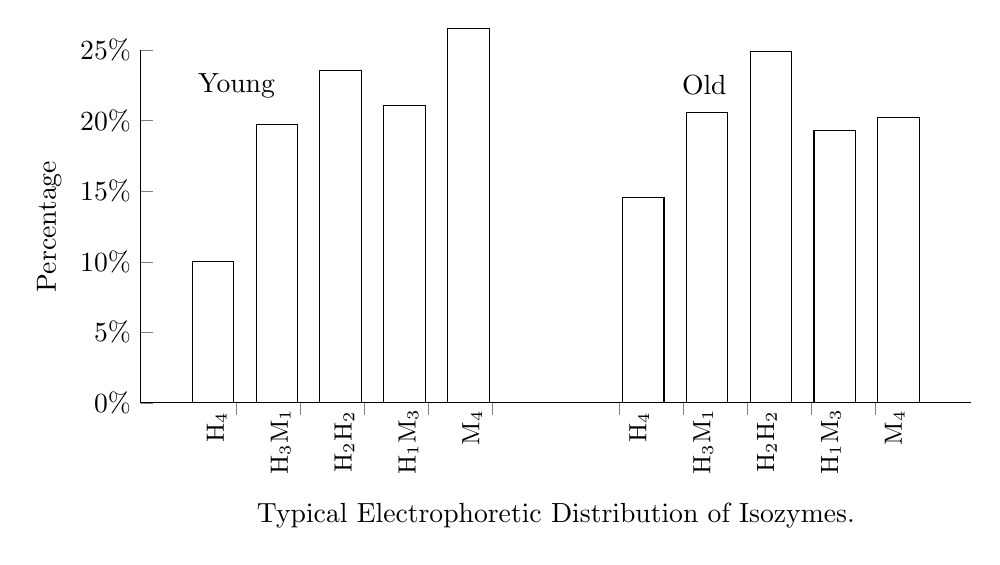
\begin{tikzpicture}
\begin{axis}[
    ybar,
    bar width=15pt,
    enlarge x limits=0.15,
    ylabel={Percentage},
    xlabel={Typical Electrophoretic Distribution of Isozymes.},
    ytick={0,5,10,15,20,25},
    yticklabels={0\%,5\%,10\%,15\%,20\%,25\%},
    ymin=0,
    ymax=25,
    axis lines*=left,
    xtick={1,2,3,4,5,7,8,9,10,11},
    xticklabels={,,,,,,,,,,}, 
    x tick label style={font=\small},
    width=\linewidth,
    height=0.5\linewidth,
    legend style={draw=none},
    clip=false,
    xlabel style={yshift=-5ex}
]

\addplot[fill=white, draw=black] coordinates {
    (1,10.042735042735043)  
    (2,19.71153846153846)  
    (3,23.55769230769231)   
    (4,21.04700854700855)  
    (5,26.549145299145305)   
};

\addplot[fill=white, draw=black] coordinates {
    (7,14.529914529914532)  
    (8,20.566239316239322)  
    (9,24.893162393162395)  
    (10,19.284188034188038) 
    (11,20.219017094017094)  
};

\node[rotate=90, anchor=south] at (axis cs:1,-1.75) {\small $\mathrm{H}_4$};
\node[rotate=90, anchor=south] at (axis cs:2,-2.75) {\small $\mathrm{H}_3\mathrm{M}_1$};
\node[rotate=90, anchor=south] at (axis cs:3,-2.75) {\small $\mathrm{H}_2\mathrm{H}_2$};
\node[rotate=90, anchor=south] at (axis cs:4,-2.75) {\small $\mathrm{H}_1\mathrm{M}_3$};
\node[rotate=90, anchor=south] at (axis cs:5,-1.75) {\small $\mathrm{M}_4$};

\node[rotate=90, anchor=north] at (axis cs:7,-1.75) {\small $\mathrm{H}_4$};
\node[rotate=90, anchor=north] at (axis cs:8,-2.75) {\small $\mathrm{H}_3\mathrm{M}_1$};
\node[rotate=90, anchor=north] at (axis cs:9,-2.75) {\small $\mathrm{H}_2\mathrm{H}_2$};
\node[rotate=90, anchor=north] at (axis cs:10,-2.75) {\small $\mathrm{H}_1\mathrm{M}_3$};
\node[rotate=90, anchor=north] at (axis cs:11,-1.75) {\small $\mathrm{M}_4$};

\node at (axis cs:1,22.5) {Young};
\node at (axis cs:8.325,22.5) {Old};

\end{axis}
\end{tikzpicture}

\begin{center}
  Mean \% of H$_{4}$:
\end{center}

\begin{center}
  \begin{tabular*}{0.8\linewidth}{@{\extracolsep{\fill}} c c c c}
    ~ & S & Y & P\\
    12 Animals & 14.3 & 10.7 & 0.05\\
    (6 old, 6 & ~ & ~ & ~\\
    young) & ~ & ~ & ~
  \end{tabular*}
\end{center}

\begin{center}
  Total LDH Activity in B-B Units per ml.:
\end{center}

\begin{center}
  \begin{tabular*}{0.8\linewidth}{@{\extracolsep{\fill}} c c c}
    S & Y & P\\
    1700 & 1950 & 0.05
  \end{tabular*}
\end{center}

\noindent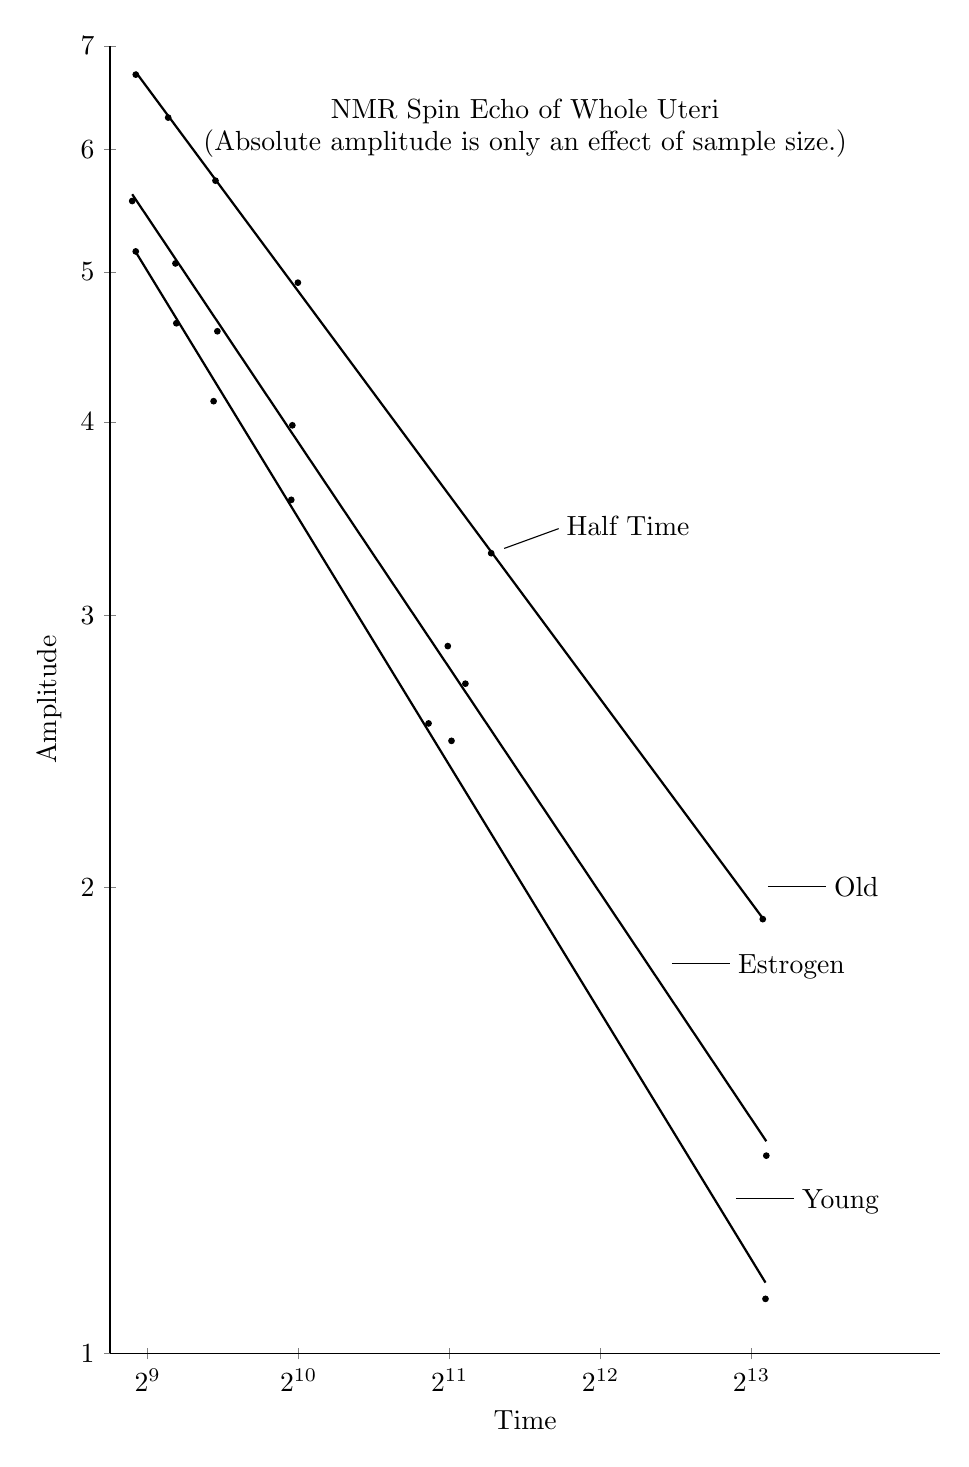
\begin{tikzpicture}
\begin{axis}[
    height=1.5\textwidth,
    width=\textwidth,
    axis x line=bottom,
    axis y line=left,
    axis line style={-},
    enlarge x limits=0.05,
    xmode=log,
    ymode=log,
    xmin=512,
    xmax=16384,
    ymin=1,
    ymax=7,
    ytick={1,2,3,4,5,6,7},
    yticklabels={1,2,3,4,5,6,7},
    xtick={512,1024,2048,4096,8192},
    xticklabels={2$^{9}$,2$^{10}$,2$^{11}$,2$^{12}$,2$^{13}$},
    minor tick num=0,
    xlabel={Time},
    ylabel={Amplitude}
]

\addplot[only marks, mark=*, mark size=1pt, color=black] coordinates {
(484.473392796994, 5.154371404524182)
(583.7664022298974, 4.631726306379266)
(692.7033586920346, 4.124722936292416)
(989.5959201130876, 3.56152022889325)
(1858.9321760543821, 2.553555376667845)
(2065.2799963287357, 2.4881773489912424)
(8732.88089123549, 1.0845901137960103)
};

\addplot[no markers, black, thick] table [
            y={create col/linear regression={y=Y}},
        ] {
            X Y
484.473392796994 5.154371404524182
583.7664022298974 4.631726306379266
692.7033586920346 4.124722936292416
989.5959201130876 3.56152022889325
1858.9321760543821 2.553555376667845
2065.2799963287357 2.4881773489912424
8732.88089123549 1.0845901137960103
        }; 

\addplot[only marks, mark=*, mark size=1pt, color=black] coordinates {
(476.6543885636081, 5.555944992854687)
(581.3915572955749, 5.063046392407869)
(704.8402424186651, 4.577074560598036)
(994.4981823178825, 3.9798454712667004)
(2030.4584265600981, 2.865102603754915)
(2201.54328499399, 2.709153812211149)
(8766.200585647728, 1.342192620230919)
};

\addplot[no markers, black, thick] table [
            y={create col/linear regression={y=Y}},
        ] {
            X Y
476.6543885636081 5.555944992854687
581.3915572955749 5.063046392407869
704.8402424186651 4.577074560598036
994.4981823178825 3.9798454712667004
2030.4584265600981 2.865102603754915
2201.54328499399 2.709153812211149
8766.200585647728 1.342192620230919
        }; 


\addplot[only marks, mark=*, mark size=1pt, color=black] coordinates {
(484.5533808541257, 6.705770062873648)
(562.3578003154925, 6.290533457111426)
(698.7598691365937, 5.726809780461477)
(1020.1143273528011, 4.920255941710608)
(2477.908979070812, 3.2897529295615016)
(8624.803425059117, 1.9087671087524056)
};

\addplot[no markers, black, thick] table [
            y={create col/linear regression={y=Y}},
        ] {
            X Y
484.5533808541257 6.705770062873648
562.3578003154925 6.290533457111426
698.7598691365937 5.726809780461477
1020.1143273528011 4.920255941710608
2477.908979070812 3.2897529295615016
8624.803425059117 1.9087671087524056
        }; 




    \draw [shorten >=2.5pt, shorten <=5pt] (7155.206427666167, 1.2587612021305639) -- ++(0:1cm) 
    node[
      anchor=west,
      align=left,
      text depth=0ex,
      inner sep=0pt,
      line width=1pt
    ] {Young};

        \draw [shorten >=2.5pt, shorten <=5pt] (5332.0033277324565, 1.7861805824247037) -- ++(0:1cm) 
    node[
      anchor=west,
      align=left,
      text depth=0ex,
      inner sep=0pt,
      line width=1pt
    ] {Estrogen};

        \draw [shorten >=2.5pt, shorten <=5pt] (8281.06371761685, 2.002608639918147) -- ++(0:1cm) 
    node[
      anchor=west,
      align=left,
      text depth=0ex,
      inner sep=0pt,
      line width=1pt
    ] {Old};

            \draw [shorten >=2.5pt, shorten <=5pt] (2477.908979070812, 3.2897529295615016) -- ++(20:1cm) 
    node[
      anchor=west,
      align=left,
      text depth=0ex,
      inner sep=0pt,
      line width=1pt
    ] {Half Time};

   \node at (rel axis cs:0.5,0.95) {NMR Spin Echo of Whole Uteri};

   \node at (rel axis cs:0.5,0.925) {(Absolute amplitude is only an effect of sample size.)};

\end{axis}
\end{tikzpicture}

\begin{center}
  Harderian fluorescence:
\end{center}

\begin{center}
\noindent\hspace*{-0.175\linewidth}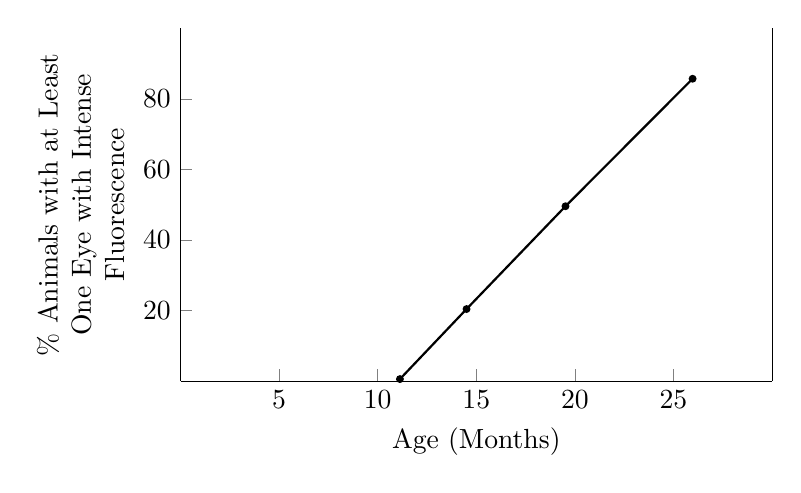
\begin{tikzpicture}
\begin{axis}[
    width=0.75\linewidth,
    height=0.5\linewidth,
    axis lines*=box,
    axis x line*=bottom,
    axis line style={-},
    xtick={5,10,15,20,25},
    ytick={20,40,60,80},
    ytick pos=left,
    xmin=0, xmax=30,
    ymin=0, ymax=100,
    ylabel={\% Animals with at Least\\One Eye with Intense\\Fluorescence},
    xlabel={Age (Months)},
    ylabel style={align=center},
    clip=false
]

\addplot[mark=*, mark size=1pt, thick] coordinates {
    (11.127879886098887, 0.5627750453016063)
    (14.505565622573128, 20.409008542583493)
    (19.524203986538957, 49.546725342997675)
    (25.970748123220297, 85.67952368625423)
};

\end{axis}
\end{tikzpicture}

\end{center}

Approximate incidence of red eye fluorescence with age in months. 25 animals.

\begin{center}
NMR Spin Echo:
\end{center}

The NMR spin echo results are similar to those of Damadian
(1971) comparing tumor with normal tissue, and of Hazelwood (1971),
comparing fetal with mature tissue. The results suggest that
senescent uterine water is more bulk-like than that of young uterus,
as tumor and fetal tissue water is more bulk-like than that of normal
and mature tissues.
\chapter{Discussion}

\epigraph{\centering ``Every statement implies a metaphysic.''}{-- A. N. Whitehead}

\section{The Paradigm Problem}

Even seemingly simple and ``straight-forward'' problems and solutions are ultimately questions of probability, and interpretation is present in the most ``objective'' treatment of a question (Tart, 1972). A more complex problem requires a more complex context if a similar degree of ``objectivity'' is to be maintained. Whenever a paradigm is left, the question of interpretation becomes more apparent.

This thesis begins by questioning the paradigm of ``aging as decline'' of hormone concentration and metabolic rate. That paradigm was based on certain gross and organismic observations, and is valid with with regard to androgenic, luteal, and certain adrenal hormones, at least in most mammals, and with regard to whole animal oxygen consumption per unit of tissue, and probably even with regard to mitochondrial respiration. However, it lacks generality. Highlights from a large literature regarding the physiology of aging are presented in the introduction, to show that a contrary, and much more general, paradigm exists, which can be stated approximately as ``in aging and other distress conditions, typical shifts of metabolic pathways occur.'' Measurements that only seem peculiar when considered in the former paradigm, may be definitive in the latter. The typical shifts of metabolism include:

\begin{center}
\begin{adjustwidth}{0.1\linewidth}{0.1\linewidth}
\begin{itemize}[label={}, leftmargin=*, rightmargin=0pt]
    \item a)~``Damaged respiration'' in the sense of a decreased efficiency of phosphorylation, or excessive hydrolysis of ATP, by high ATPase activity, which can result from mitochondrial damage;
    \item b)~Compensatory glycolytic phosphorylation;
    \item c)~Given mitochondrial damage and NADH production in glycolysis, a necessary step in compensation is the oxidation of NADH, for example by LDH, or peroxidase, of ``age-pigment-related NADH oxidase.'' Either lactate formation, or oxygen consumption, or both, or another kind of oxidation, must increase if glycolysis is to proceed.
\end{itemize}
\end{adjustwidth}
\end{center}

This paradigm forms an interpretive link between the various ``distress conditions,'' and suggests that low oxygen tension will be a factor in these various conditions. The literature on mammalian loss of fertility under many conditions, e.g., x-irradiation, estrogen treatment, adrenaline treatment, senescence, vitamin E deficiency, progesterone deficiency, intrauterine devices, etc., is remarkable for the great similarities that exist in such diverse conditions. Estrogen action is the most common and easily manipulable of these conditions, and so each of the other conditions tends to be described as ``estrogenic.'' Knowledge regarding the states in which estrogen may be bound within the uterus is not adequate to provide a sound bases for its extraction and unambiguous assay. Whether these conditions that prevent gestation actually increase estrogen concentration in the uterus, or merely mimic it, is still debatable. The available metabolic information about the various ``distress conditions'' indicates that oxygen wastage is likely to be a common factor; data on embryos' requirement for oxygen \textit{in vitro} show that oxygen deprivation \textit{in utero} could be responsible for pregnancy wastage. The new paradigm suggests the hypothesis of loss of fertility through excessive reduction of oxygen, as a normal feature of aging, as well as in the various other ``distress conditions.'' All aspects of the hamster uterus that have been measured are consistent with this. The old paradigm does not unambiguously predict any of the observed age changes. To make it do so requires a complex series of \textit{ad hoc} assumptions, each one to explain away as ``non-estrogenic'' a change which to this point had been considered to be estrogenic. One clear prediction that it makes is that the senescent uterus will \textit{not} have an elevated metabolic rate. This is refuted by the observations, especially the TTC reduction.

Another clear prediction made by the old paradigm is that senescent sterility and estrogen-induced sterility will not act by the same mechanism, since senescent sterility is conceived of as an effect of estrogen deficiency, exactly the opposite of an estrogen excess. However, the data shows that senescence lowers oxygen tension, just as estrogen treatment does.

It is remarkable that, in spite of \textit{in vitro} studies that show sensitivity to of mammalian embryos to changes in oxygen tension, the issue has been almost entirely ignored in studies of fertility, and has never previously been considered in relation to senescent sterility. Even percentages of oxygen higher than atmospheric can be limiting to embryos implanting \textit{in vitro}, suggesting that implantation is especially sensitive to oxygen deficiency. Implantation is also the main point of damage in the various ``distress conditions,'' as far as the question has been investigated.

A paradigm by definition is open-ended enough to allow for further development, and so can never be overturned by data or reasoning, but it can become increasingly untenable. The smaller question, however, of whether oxidative changes are adequate to account for embryonic retardation, non-implantation, and resorption can be more decisively answered, because the less complex question calls on a less complex interpretive context.

The observations require rejection of the view that an oxygen deficiency cannot occur in the uterus from common physiological causes. Hypoxia has been proposed as the cause of abortion following vasoligation, but it has been generally believed that only such gross interference with circulation could produce sufficient hypoxia. That the cause can be physiological is indicated by the increased metabolic rate.

Beyond this, the observations characterize the senescent uterus as being in a very common physiological state, which can be called a ``distress state.'' The causal relation between age and the other states is discussed on the basis of the literature. Senescence is physiological, and the physiology is such that sterility must result.

The correspondence of the changes in the senescent uterus to changes in the other ``distress states'' supports the view that the changes are patterned, paradigmatic, coherent, and meaningful metabolic changes. Although the pathway details are not completely known, the existence of compensatory glycolysis and non-mitochondrial oxidation have been well established in various tissues.

\section{The Senescent State}

There is considerable evidence that the estrogen/progesterone ratio, or estrogen/17-keto steroid ratio, increases with age, at least in mice, rats, rabbits, and women, and that this change has metabolic effects similar to treatment with exogenous estrogen. However, irritation, low thyroid, excessive copper absorption, etc., probably could increase the estrogen effect without necessarily affecting the concentration of circulating estrogens. To find in senescence the metabolic state associated with estrogen treatment is interesting more for the possible effects of this state on functions such as implantation, than for its corroboration of a suspected excess of estrogen. The generality of this ``distress state'' of metabolism is intrinsically interesting.

\section{Enzymes}

Many enzymes, including ATPase, spermidine synthetase, alkaline phosphatase, NADH-oxidase, $\beta$-glucuronidase, sulfatase, peroxidase, hexokinase (Gross, 1961), malate dehydrogenase (Wilson, 1969), glucose-6-phosphate dehydrogenase and 6-phosphogluconate dehydrogenase (Schmidt, et al., 1967), lactic dehydrogenase, and ornithine decarboxylase (Kaye, et al., 1971), change in activity under the influence of estrogen, but a few are especially important in relation to oxidative metabolism. An apparent increase of cytochrome oxidase following estrogen treatment turned out to be peroxidase (Lucas, et al., 1955).

LDH was considered to be an especially suitable enzyme to study in relation to implantation because its total activity and isozyme composition are known to reflect oxygen concentration and degree of estrogenic stimulation, and to relate to the tissue's disposition of lactate and pyruvate (Johansson, 1966; Battelino, et al., 1971; Goodfriend and Kaplan, 1964; Dawson, et al., 1964). The enzyme can also function as a potential ``transhydrogenase'' system (Sanwal, et al., 1970; Young, 1961), and thus is in a position to regulate the glucose-6-phosphate oxidation pathway of carbohydrate metabolism. Also, the equilibrium

\[
  \ce{lactate + NAD+ <=> pyruvate + NADH + H+}
\]

\noindent implies that the reaction proceeds toward lactate formation, the pH will tend to rise. In many tissues the ratio of lactate/pyruvate is much smaller than the chemical equilibrium, probably because of oxidative competition for the NADH (Olson, 1963). Restricting oxygen would probably allow the reaction to move farther toward equilibrium, with a consumption of protons. Elevated pH tends to weaken other controls (e.g., the inhibiting effect of ATP, involved in the Pasteur effect) over phosphofrutokinase (Racker, 1972) which is an important control point in glycolysis. Waddell (1969) has pointed out that the addition of glucose to cancer cells tends to raise the intracellular pH, as the cells form large amounts of lactate. High pH has been observed to increase the rate of lactate formation without increasing respiration (Tobin and Mehlman, 1971). In aged rats, intracellular pH may be elevated (Comolli, 1971) as well as lactate production in certain tissues (Angelova-Gateva, 1968). The NAD$^{+}$/NADH ratio also controls the rate of glyceraldehyde-3-phosphate oxidation (Racker, 1972). LDH is thus in a position to exercise extensive control over glycolysis, possibly providing a mechanism for interfering with the Pasteur effect (which is decreased under the influence of estrogen: Greenstein, 1954). The LDH isozyme ratio may be of importance not only for determining the availability of pyruvate for oxidation, but for regulating other pathways. (Considering the low pO$_{2}$ of senescent or estrogen dominated hamster uterus, and the requirements of spermatozoa for oxygen [Nevo, 1965], the X isozyme in male producing spermatozoa [Stambaugh and Buckley, 1970] may relate to the lower proportion of males in senescence or estrogen treatment [Hahn and Hays, 1963]).

In the presence of very active NADH-oxidase, pyruvate and lactate might also have a ``coenzyme'' function in relation to this enzyme. Peroxidase, which is ``induced'' by estrogen, has a NADH-oxidase function (Lucas, et al., 1955), and this activity is also found in association with age pigment (Strehler, 1967).

There is a slight decrease of total LDH activity in old animals, probably not significant considering their higher proportion of connective tissue and collagen.

Oxygen tension regulates the isozyme ratio, both \textit{in vitro} and \textit{in vivo} (Clark and Yochim, 1971; Yochim and Clark, 1970; Fujisawa, 1969; Johansson, 1966). Citric acid cycle intermediates can retard the formation of isozyme ``M'' by chick heart muscle cells in culture (Cahn, 1969), but oxygen tension has its isozyme inducing effect regardless of the presence of metabolic inhibitors, including fluoroacetate, potassium cyanide, 2,4-dinitrophenol, and sodium amytal (Johansson, 1966). Because of this, it has been speculated that oxygen might act directly on the genes regulating LDH isozyme synthesis, but other methods of control, such as preferential degredation (Pruitt, 1971; Greengard, 1967) might be more fruitful to investigate experimentally, especially considering the greater lability of the ``liver'' isozyme, both in heat and cold (Zondag, 1963; Kreutzer and Fennis, 1964). Direct action of oxygen or peroxides on the labile isozyme, or an effect involving sequestering of the stabilizing coenzyme, NAD, might be mechanisms for regulating isozyme proportions. The H$_{4}$ isozyme seems to be the most lipophillic as well as the most stable, and the M$_{4}$ the least lipophillic (Kabara and Konvich, 1972). This result is implicitly predicted by the theory which relates cytoplasmic phase changes to control of enzyme activity (Peat and Soderwall, 1972).

Finding the H$_{4}$ isozyme increased with age leads to at least two or three questions:

\begin{center}
\begin{adjustwidth}{0.1\linewidth}{0.1\linewidth}
\begin{itemize}[label={}, leftmargin=*, rightmargin=0pt]
    \item 1)~Does enzyme induction by oxygen relate to the rate of consumption of oxygen, rather than to oxygen tension itself?
    \item 2)~If the function of this isozyme is to save some pyruvate for another use, rather than converting it to lactate (Lehninger, 1970), is carboxylation to oxaloacetate that use?
    \item 3)~Would it lead to a situation in which (because of H-LDH's inhibition by high concentrations of pyruvate) pyruvate carboxylase tended to become rate limiting for glycolysis?
\end{itemize}
\end{adjustwidth}
\end{center}

Although no mechanism is suggested, it is interesting that the age shift of isozymes is opposite to the shift which occurs in pregnancy, as early as day 5, when uterine oxygen consumption is known to decrease (Battelino, et al., 1971).

$\beta$-Glucuronidase is increaed in liver, uterus, kidney, and other tissues by injection of estrogen (Fishman, 1950) or various poisons, and this effect has been likened to the induction of detoxifying enzymes in the liver by their substrates. Levvy (Karunairatnam and Levvy, 1949) has offered the contrary interpretation that $\beta$-glucuronidase is merely involved in tissue proliferation, regardless of what causes the proliferation. Prolonged estrogen treatment causes an eventual decline in $\beta$-glucuronidase, as it does of the mixed function oxidases (Song and Kappas, 1968). Its decline with age in the hamster uterus thus is consistent with the view that estrogen tends to dominate uterine metabolism in senescence, but of course doesn't imply that this is what occurs. However, if its normal function in the uterus and other tissues is to conjugate and remove estrogen to prevent estrogen toxicity, then its absence in the senescent uterus would suggest an explanation for other physiological changes that occur in the uterus with age. If estrogen no longer turned over in the uterus, then a much smaller supply could raise the uterine content, Estrogen treatment is known to ``induce'' large amounts of the estrogen binding protein (Kraay and Black, 1970), as well as reducing the progesterone binding capacity of the uterus (Armstrong and King, 1971). Post-menopausal women have at least as high a concentration of uterine ``estrogen receptor'' protein as do young women (McGuire, et al., 1972; Trams, et al., 1971).

$\beta$-Glucuronidase is known to have an \textit{in vitro} transferase function (e.g., transfer of glucuronic acid from phenolphthalein to an alcohol) besides it common hydrolytic function (Fishman and Green, 1957). It has been shown to have a slow synthetic function \textit{in vitro} (Florkin, 1940). Fishman (personal communication) feels that an \textit{in vivo} conjugating (transferase) function is plausable, considering the similar role of a ``hydrollytic'' enzyme such as glucose-6-phosphatase. $\beta$-Glucuronidase is so abundant in smooth endoplasmic reticulum that it is considered likely to be a structural protein (Wakabayashi, 1970).

CATALASE: Catalase activity of the uterus is interesting because it is believed to relate to the cytochrome system (Deisseroth and Dounce, 1970), is lower in the female, at least in some species (Adams, 1965), ans since either its rate of synthesis or rate of degradation appears to change with age in mouse liver (Baird and Samis, 1971). The fact that its activity is lowered by riboflavin deficiency (Adams, 1965), and by serum or tissue extract from animals with tumors (Nakahara and Fukuoka, 1959), and is lower in females, suggests that its level will correspond to the amount of energy derived form mitochondrial oxidation. A similar extract is an abortifacient. The lower level in the aged uterus would not be particularly interesting if oxygen consumption were lower in that tissue. Since oxygen consumption tends to be higher, low catalase activity suggests that the oxidation may not be occurring in the usual way.

PEROXIDASE: The fact that estrogen activates the NADH-oxidase function of peroxidase, which itself is ``induced'' by estrogen (Lucas, et al., 1955; Yokota and Yamazaki, 1965; Jellink and Lyttle, 1971; Temple, et al., 1959; Hollander and Stephens, 1959; Beard and Hollander, 1962) suggests that in the uterus peroxidase may be involved at an early stage in the process of cell activation by estrogen. Vitamin E, which is known to inhibit peroxidation, has anti-estrogenic effects, including inhibition of the formation of the estrogen-dependent uterine age pigment, which is associated with NADH-oxidase activity, and which is generally considered to result from peroxidation of lipids and proteins (Elftman, et al., 1949).

VITAMIN E: Two classical symptoms of a vitamin E deficiency are increased tissue oxygen consumption (Houchin, 1942) and anemia (Fitch, 1968). The degree of stability of erythrocytes in the presence of oxidants, such as hydrogen peroxide, is an indication of the vitamin E status of the animal. Vitamin E has an anti-oxidant function, but other properties are also believed to be involved in its vitamin activity. It increases the viscosity of protein solutions (e.g., albumin), apparently by causing a more extended conformation of the protein. Such a physical or mechanical property, as well as a chemical anti-oxidant property, could be involved in its anti-hemolytic effect, and in its ability to stabilize other ``membrane'' systems, such as lysosomes (McCay, et al., 1971). It lowers the extractability of muscle proteins (Matusis, 1970). The enzymes of vitamin C synthesis in microsomes are inactivated by lipid peroxides, and preserved by added $\alpha$-tocopherol (Chatterjee and McKee, 1965). Estrogen's effects on vitamin C synthesis, $\beta$-glucuronidase (of lysosomes), and pigment formation may be produced by a common structural event. uterine age pigment requires estrogen for its development, but vitamin E treatment prevents its formation (Kaunitz, et al., 1948; Atkinson, et al., 1949). If hemes, or other porphyrins, are related to the lipofuscins or age pigments, they may be responsible for the NADH-oxidase activity that Bjorkerud (Strehler, 1967) found associated with the pigments. The same hemolysis which lends to vitamin E deficiency anemia could therefore also be responsible for the increased oxidation of vitamin E deficiency. Since hypoxia stimulates porphyrin synthesis (Falk, et al., 1959), oxygen wastage by porphyrins would tend to be a positive feedback process. The oxidase activity of age pigment granules is cold-inactivated (Bjorkerud and Cummins, 1963), which is consistent with the theory of pathway regulation by ``structural temperature'' (Peat and Soderwall, 1972). If estrogen's action is intrinsically realted to a hypoxic state, this could also explain the fact that porphyrins are synergistic with estrogen, and similarly could explain the occurrence of porphyrins mainly in female and cancer-prone rodents (Strong, 1942; Figge, 1942). Vitamin E is known to lower serum bilirubin related to liver damage (Schwarz, 1949).

The circulatory availability of oxygen, as well as the metabolic disposition of oxygen, may be directly related to the vitamin E status of the animal. Adaptive hyperemia in several glands has been found to result from the action of peptide kinins, produced by proteolytic kallikreins (Schachter, 1969). Small molecule inhibitors (e.g., Trasylol, $\varepsilon$-amino caproic acid) are known, as well as the protein inhibitors, of the kallikreins and other proteolytic enymes (cathepsins, trypsin). Age, x-irradiation, and estrogen have been implicated in various ways in proteinase inhibition. The ``Schute test'' (Schute, 1937; de Oliveira, 1949), a measure of the level of serum proteolytic inhibitory activity, clearly shows that a vitamin E deficiency increases the inhibition of proteolytic enzymes. The presence of inhibitors would tend to suppress formation of kinins, the local ``inflammatory'' vasodilators, and would also interfere with clot removal.

The hamsters that were given vitamin E in very large doses showed chronic leucocytic vaginal smears, as in rats given daily doses of progesterone (Labhsetwar, 1970).

A vitamin E deficiency causes muscles of rabbits (Morgulis and Oscheroff, 1937) to increase their concentration of ``extracellular'' ions, especially Na$^{+}$, Cl$^{-}$, and Ca$^{++}$, suggesting a possible loss of organic ions, as well as an energy loss: creatine phosphate may be largely responsible, since vitamin E deficiency causes creatinuria.

The observations of Thorneycroft and Soderwall (1969) regarding fewer and smaller corpora lutea in senescent hamsters may relate to the observations of Lecoq and Insidor (1949) that vitamin E deficient rats have no corpora lutea.

Progesterone's effect on Na$^{+}$, Cl$^{-}$, and Ca$^{++}$, and water is similar to that of vitamin E, and opposed to estrogen's effect. The most sensitive demonstration of vitamin E's anti-estrogen effect is probably Leqoc's (1949) on uterine chronaxy.

Vitamin E requirements increase with age (Fuhr, et al., 1949; Ames and Ludwig, 1964; P'an, et al., 1949; Emerson and Evans, 1940) and a deficiency acts mostly to block implantation (Blandau, et al., 1949).

\section{Oxygen Consumption}

A likely source of error in measuring tissue oxygen consumption (besides the problem of balancing cell damage in thin slices or minces against limited diffusion in thicker slices: Jusiak, 1970) is in neglecting for other gaseous metabolites (Dudka, et al., 1971; Maharajh and Walkley, 1972) than oxygen and carbon dioxide, of which ammonia is likely to be the most important by far. Tashiro (1922) observed ammonia production in nerve and muscle, which increased when the tissue was stimulated. Needham (1942) wrote that ammonia is not likely to be produced by embryonic tissue unless sufficient carbohydrate is not available, implying that it results from protein catabolism. A popular contemporary argument (Lowenstein, 1972) is that ammonia emission results from the activity of adenylate deaminase, but in amny cases glutamic dehydrogenase seems a more likely enzyme. In estrogen stimulation protein synthesis and turnover are accelerated (Mueller, 1968); glutamic acid is an important link between carbohydrate metabolism and proteins, and is also closely related to synthesis of pyrroles. Aspartate, however, seems to be the first amino acid synthesized after estrogenic stimulation (Jervell, et al., 1958), probably by amination of oxaloacetate (Barker and Warren, 1966). Glutamate dehydrogenase may have alanine dehydrogenase activity when dissociated into subunits. Estrogen can regulate this dissociation and change of activity, probably by increasing the supply of NADH (Tomkins, et al., 1961). Estrogen-induced L-alanine pyruvate conversion by this form of glutamate dehydrogenase would account for some of the diversion of pyruvate into protein synthesis. Lacking carbohydrate, a reversal of the reaction could form pyruvate, with a high rate of protein catabolism and production of ammonia. (A shift of the enzyme activity away from glutamate dehydrogenase may spare glutamate for synthesis of $\delta$-levulinic acid, and porphyrins.)

Senescent uterus has reduced glycogen levels in pregnancy (Connors, 1969), and if this lack of glycogen exists in the cycling senescent uterus, or if the rate of metabolism is high in relation to available carbohydrate, aged uterus may release more ammonia than young uterus. \textit{In vitro}, where small glycogen deposits may be quickly consumed and no external glucose is provided, the tissue with the highest metabolic rate will probably release the most ammonia, and if this is not taken into account, the manometric method will read this a diminished oxygen consumption. In the first measurements, samples often showed negative ``oxygen consumption,'' and this occurred more often with senescent tissue, especially myometrium, and probably was intensified by delay in preparing the tissue. Although the literature on uterine oxygen consumption does not mention this problem, it may be a general factor in measurements of oxygen consumption. When sulfuric acid was added to the vessel side arms, oxygen consumption measurements became consistently positive and rates became more consistent, especially in the case of senescent tissue.

Dissolved oxygen measurements would tend to show alteration in the opposite direction when ammonia is released, so additional measurements were made in the Beckman apparatus. No removal of ammonia is possible in this case, so the data should be considered only in relation to the manometric data, unless it can be assumed that the much shorter time needed to get measurement eliminates the factor if ammonia production.

Increased oxygen consumption by estrogen-activated tissue does not imply increased mitochondrial oxidation, coupled to phosphorylation or not. Lucas, et al., (1955) determined that what had been assumed to be elevated cytochrome oxidase activity was actually the NADH-oxidase activity of peroxidase. Wilson (1969) reported the puzzling observation that estrogen increased the activity of only malate dehydrogenase of all the citric acid cycle enzymes, and that others may have decreased. It is interesting that MDH is one of the few enzymes known to increase in some tissues in senescence (Finch, 1972). The carboxylation of pyruvate to oxaloacetate, followed by amination to form aspartic acid (Barker and Warren, 1966; Jervell, et al., 1958) may have its equivalent in this situation, viz., production of oxaloacetate for amino acid formation.

Barker, Neilson, and Warren (1966) claim that lipid synthesis, mediated by NADP$^{+}$, regulates the hexose monophosphate shunt. (Elsewhere it has been suggested how a cytoplasmic phase change could accelerate lipid synthesis: Peat and Soderwall, 1972). They found that the specific activity of glucose-6-phosphate dehydrogenase decreased significantly during an early period in which G6P and 6PG were being oxidized at an increased rate. Activation of either lipid synthesis or oxidation of NADPH would be able to stimulate this pathway.

\section{Oxygen Tension}

The measurements of intrauterine pO$_{2}$ that have been made with the Beckman microelectrode inserted through an 18 gauge arterial needle (Yochim and Clark, 1971; Mitchell and Yochim, 1968 ,1969b; Salderini and Yochim, 1967) are apparently inaccurately high. The sharp end, and additional thickness, possibly cause stil-oxygenated blood to be free into the cavity surrounding the electrode tip, where it would not be subject to oxidation by the tissue. The cyclic variation of about 20 mm. Hg pO$_{2}$ could be a further artifact, since the electrode itself reduces oxygen and will quickly lower the oxygen tension of a small volume of fluid that is not stirred. The end of the needle immobilizes a few microliters of liquid. Periodic contractions of the uterus would replace the fluid in the tip of the needle with fresh blood (or another oxygenated fluid produced by introducing the electrode) from elsewhere in the lumen. This procedure gave measurements in the hamster's uterus that were about the same as those obtained by Yochim and others in the rat, except that instead of one minute cycles, in the hamster the cycles were about three to four minutes long. Different means or maxima determined by this method would therefore reflect indirectly the rate of oxygen consumption by measuring the level of oxygen present in the blood which is released into the lumen. The rate of oxygen consumption would not be entirely unrelated to tissue pO$_{2}$ (yochin, 1971), but it would present an entirely false picture of the conditions experiences by the pre-implantation embryo.

Using the ``bare'' electrode (with stainless steel jacket, but no needle around it) with a diameter of 1.0 mm. and a blunt tip, a much lower pO$_{2}$ was measured, and there was no cyclic change that could be recorded. The oxygen tension is so low that an accurate absolute measurement is extremely difficult, but relative measurements of differences between animals can be easily and clearly made. The oxygen tensions observed are lower than any known mammalian tissue except cancer. Senescent animals' uteri had a pO$_{2}$ in the range of 0-2 mm. Hg, young animals in the range of 4-8 mm. Hg, and vitamin E treated senescent, 6-12 mm. Hg. The color of the uterus varied from maroon in the old animals to pale pink in the vitamin E treated animals; young animals' uteri were bright red.

At such low oxygen tension it might be advantageous to have hemoglobin with high oxygen affinity; it has been reported that sheep with hemoglobin A (with higher than normal oxygen affinity) are better able to withstand the abortifacient effects of estrogenic pasture than are other sheep (Obst and Seamark, 1971). A lower ``unloading tension'' would correspond to a lower tissue oxygen tension, with possibly adaptive effects, such as a more controlled or gradual release of oxygen. Oxygen consumption decreases at implantation sites in the rat uterus at the time of implantation (Suranu and Heald, 1971), and this probably causes a rise in pO$_{2}$ to levels the embryo requires. Progesterone by counteracting estrogen, may be the cause (Goodland, et al., 1953). As early as the fourth day of pregnancy there are greatly increased obstructions in the uterus, probably from increased adhesiveness of the epithelium which at this time is closing over the blastocysts. Even the ``bare'' electrode has to be forced if it travels more than a centimeter from the opening, and obviously is causing luminal bleeding. The force required was such that at one obstruction the electrode passed entirely through the wall of the uterus. before hitting an obstruction the pO$_{2}$ reading was 40 mm. Hg, which might have been high because of being near the opening, though the soft and abundant endometrium formed a seal. Beyond the obstructions the pO$_{2}$ measured 5-10 mm. Hg, or about that of the vitamin E treated cycling hamsters. The average blood would be expected to have more oxygen than the respiring tissue, but if the deeper stromal or myometrial tissue were respiring faster than the implanting epithelium, bleeding might cause a lowering of pO$_{2}$.

Yochim's system of measuring uterine luminal oxygen tension with an aterial needle may be measuring something equivalent to the ``bulk'' pO$_{2}$ in organ culture, i.e., possibly uterine fluid that has been contaminated with oxygenated blood or gas introduced with the needle, so they are possibly correct about the effect of pO$_{2}$ on LDH isozyme proportions in the uterus ,which they compare to the effects in cultured uteri.

However, the pO$_{2}$ at the surface of the cell in culture, where the effect of pO$_{2}$ on LDH isozymes is to be studied, will be much lower, becaus eof an O$_{2}$ gradient in the unstirred layer. A bare electrode, able to contact the epithelial tissue in the uterus, and less likely to cause bleeding, would probably more closely approach the pO$_{2}$ actually experienced by tissue either \textit{in vivo} or in culture.

The pO$_{2}$ Yochim's group measured would not, according to Needham's review (1931), be low enough to approach limitation of embryonic development. However, when the lumen ``surface'' pO$_{2}$ is measured, by the bare electrode, the tension is seen to be lose to that which limits respiration and development of embryos; the actual pO$_{2}$ the embryo experienced in the experiments reviewed by Needham is not known, nor is the actual pO$_{2}$ in the old hamster's uterus, since it is at the extreme lower limit of the measuring system's capacity. A better technique is needed, to determine the real minimum.

\section{TTC Reduction}

The reduction of triphenyl tetrazolium chloride is considered to reflect dehydrogenase activity (Racker, 1955; Novikoff, 1959) or the cell's reductive capacity, including substrate availability, and is believed to be one of the most sensitive indicators of estrogenic stimulation. It is known to accurately correspond to QO$_{2}$ in many tissues (Cascarano and Zweifach, 1955). Martin (1959) has reported that the TTC reducing response of the ovariectomized mouse vagina to exogenous estrogen is linear in relation to dosage from about two picograms of estradiol per mouse up to about one microgram. Estrogen increased phosphorylase activity (Takeuchi, et al., 1962) and ATPase activity, so would tend to release inhibition of glycotic enzymes while providing increased amounts of glucose. Ammonia is a very effective activator if phosphofrutokinase, and may be produced by cell activation (Lowenstein, 1972). The production of NADH would therefore be increased. The earliest effect of estrogen may be on glycolysis, rather than on respiration (Roberts and Szego, 1953). Since estrogen causes ``induction'' of peroxidase, which has NADH oxidase activity (for which estrogen serves as a coenzyme: Beard and Hollander 1962), at least part of the increased NADH would tend to reduce oxygen by this short-circuit route, increasing oxygen consumption without necessarily increasing usable oxidative energy production. That is, an extramitochondrial uncoupling of oxidative phosphorylation could occur though these known ezymic effects of estrogen. Whatever the mechanism, increased oxygen consumption must lower the pO$_{2}$ of a tissue of circulation doesn't increase proportionally. According to Yochin, et al., (1971) circulation doesn't increase as fast as the mas of tissue increases, under estrogenic stimulation. With the rapid ``uptake'' of water (or possibly metabolic production of water) immediately after estrogen treatment, the average distance of cytoplasm from capillaries must increase, which would possibly decrease the efficiency of tissue oxygenation.

The fact that the senescent hamster uterus shows a distinctly increased TTC reduction is probably the best evidence that senescent sterility is the result of an active physiological process (or malfunction). Schultz (1964, 1965, 1966, 1967, 1968) has found that strain differences in rats suggestive of estrogen differences correlate with fertility and TTC reduction. Selection for large bodies produced low uterine TTC reduction and large litters, while selection for small bodies produced high uterine TTC reduction, and small litters. He also found increased TTC reduction at the time of senescent litter loss by resorption in rats.

Racker's (1955) ``nothing dehydrogenase'' of well-dialyzed protein fraction, which give a string nitroprusside reaction, reduces NAD or NADP without the addition of substrate, and the reduced nucleotide can then reduce tetrazolium. Racker and others have suggested that protein SH groups are the source of this reducing capacity. The present tendency is probably to assume that starches or fats contaminate the protein fraction and provide the reductive capacity. However, G. Ungar (1957, 1959) has presented some evidence to support the view that cell excitation involves an increase of protein SH groups, resulting from conformation changes or ``partial denaturization'' after excitation or hormone treatment. The technique of determining uterine protein SH concentration is very hard to use reliably, but might eventually be useful to study the more exact nature of the uterine reducing capacity which changes with age and estrogen treatment.

\section{Age Pigment}

Uterine ``age pigment,'' which develops in the presence of estrogen and vitamin E deficiency (Kaunutz, et al., 1949), is not noticeably soluble in ethanol, benzene, benzyl benzoate, acetone, or chloroform, but is highly soluble in alkaline pyridine solution, which is an excellent bile pigment solvent, and is partly soluble in ether, which is also a solvent for certain bile pigments (With, 1968), and the spectrum is somewhat similar to that of a blood extract. The presence of an ether soluble fraction of bile pigment of a certain magnitude in human serum is considered to be indicative of cancer (With, 1968). Bjorkreud (1964) has observed that age pigment has NADH oxidase activity, and contains the same heme group. Aged uteri (Zinkat, 1931) contain remarkably large amounts of iron, which might be bound by the hemes. The fact that the pigments appear under conditions in which red blood cells are hemolyzing rapidly, further supports the possibility that they are porphyrin-related (Gyorgy and Rose, 1949). Bjorkerud (1964) also observed that this NADH oxidase activity of the pigment is cold-inactivated, which tends to support the theory of entropic activation of oxygen consumption (Peat and Soderwall, 1972).

\section{NMR}

The evidence is very good that water near interfaces is structured differently from bulk water (Drost-Hansen, 1971, 1972). Probably the most dramatic demonstration was Shereshevsky's (1928) experiment showing very low vapor pressure of the waster in capillary tubes. What is still in dispute is whether the particular structure induced by a surface represents an intrinsic ``phase'' or crystal-like state of water (Drost-Hansen, 1971, 1972), or whether the particular repeating pattern of the surface (such as a macromolecule) imposes its structure onto the water (Ling, 1972). It has been pointed out that the enzyme biochemists (the ``Pauling School'') emphasize the role of ionic side chains of proteins in ordering (or binding) water, while the fiber chemists emphasize the role of the protein backbone (Lin, 1972). Since estrogen stimulation involves a decrease in protein, DNA, and RNA concentration, because of the great increase in water concentration, the average distance of intra-cellular water from macromolecular surfaces must increase, and this should mean that the water molecules experience fewer restrictions of orientation. High resolution NMR spectra show a distinct broadening of the water line in tissue, relative to bulk water, and less broadening (with a shift upfield) in estrogen-treated uterus than in atrophic uterus from ovariectomized hamsters. Old uteri were not significantly different from young uteri, and both were intermediate between tissue from ovariectomized and estrogen-treated animals. The method, of course, can't determine the quantity of extracellular and intracellular water, unless their movement or shielding is very different, and this apparently is not the case. Diffusion, proton exchange, paramagnetic ions, and lipids are all probable sources of error in this method.

Spin echo NMR can eliminate the possibility that the line broadening results from proton exchange, and shows a slight difference between old and young uteri ,as well as between estrogen-treated and untreated young animals, with young uteri showing the greatest difference from bulk water. The old uteri, by being intermediate between younger uteri and bulk water, are somewhat analogous to the malignant tumors in Damadian's study (1971). Even very dense connective tissue (rat knee joint) responds to irritation by a similar change in water relaxation time, without a large uptake of water (Rokityanskiy and Yakimov, 1971).

\section{Harderian Fluorescence}

This strain of hamsters apparently has less active porphyrin secretion from the Harderian glands than do many other rodents, unless their diet is simply richer in B vitamins. A B vitamin (especially pantothenic acid) deficiency is known to cause increased porphyrin secretion by the Harderian glands. Seince World War II, animal feeds have become more standardized and are generally supplemented with adequate vitamins, and this may account for the loss of interest in the Harderian glands and their porphyrin secretions. Most (about 80\%) barely senescent (14 months) hamsters that have been examined in this la showed no fluorescence of the eye socket, or only a weak green fluorescence. Beyond this age, however, the typical bright red fluorescence becomes more common. By the time their body weight begins to decrease, which is usually after 15 months, most of the females showed some red fluorescence, but no male did. This is consistent with the observations of Strong (1942) and Figge (1942) regarding the relation of the secretion to estrogen (no males showed fluorescence) and possibly to the likelihood of an animal to develop cancer. Its appearance around the time of reproductive senescence suggests that the liver function may be decreasing at this time, and that the pigment may be related to the altered uterine metabolism.

Porphyrins are synergistic with estrogen, as well as with carcinogens (Strong, 1942; Figge, et al., 1942; Bittner and Watson, 1946, Kennedy, 1970), and the pyrroles and porphrins are also conjugated by the liver for excretion via the kidneys. With liver damage, they accumulate, causing porphyria (With, 1968). at least in rodents, concentration of porphyrins in the Harderian glands corresponds to estrogen levels and to the tendency to develop cancer, as well as to deficiencies of the B vitamins essential for liver conjugation (Figge, 1944; Hoffman, 1972).

\section{Uterine Weight, Water Content, and Thickness}

Organ weight has been said to be a more sensitive index to metabolic change than any other single condition (Criscuolo, et al., 1955; Rusin, 1971). All dimensions of the hamster uterus that were observed, diameter, thickness of endometrium and myometrium, and total weight, increased with age, but there was no significant difference between young and old endometria's water content.

Though all parts of the old uterus are enlarged, the biggest change with age appears to be the thickness of the myometrium. A large part of the collagen that accumulates with age is in the myometrium (Loeb, 1939).

Estrogen inhibits collagenase (Jeffery, et al., 1971; Woessner, 1968) and increases collagen synthesis (Henneman, 1968; Kao, et al., 1964). Loeb (1939) found that estrogen and age both cause collagen accumulation in the uterus. Schaub (1965) found a three-fold increase of uterine collagen in the aged rat, and observed the same age changes (crosslinking) that occur in other tissues.

Finn (1963) found that collagen accumulates in mouse uterus with age, both in a barren uterine horn and in a repeatedly pregnant horn, when the mouse was unilaterally ovariectomized. This weakens the arguments that maintain that collagen formation is largely the result of mechanical stress.

Alkaline phosphatase activity increases with estrogenic stimulation. Therefore, if excessive estrogenic stimulation is responsible for the failure of implantation in senescent animals because of an inadequate level of progesterone, alkaline phosphatase activity should be demonstrable.

In slides prepared by T. J. Connors for a study of enzyme changes in implantation (1969), at all times examined--days 3$\frac{1}{2}$, 4, 4$\frac{1}{2}$--the epithelium of the senescent uterus was more intensely stained. The senescent stroma was more intensely stained on day 4$\frac{1}{2}$, but on day four it was in several cases more lightly stained than in the young.

Since the decidual cell reaction (to an artificial stimulus, viz., the injection of air: Stockton, 1972) is delayed by about twelve hours in the old hamster (and also fails to produce a weight increase as great as in the young animal), this difference in stromal alkaline phosphatase probably corresponds to that delay. Horikoshi and Weist (1971), among others, have attributed ``uterine refractoriness'' to a small progesterone/estrogen ratio.

The epithelial reaction, however, seems to reflect a chronic difference. The senescent myometrium stains nearly as much as the endometrial stroma, but the young myometrium is almost unstained, on all days examined. Again, this suggests a possible chronic difference in degree of ``estrogenic'' stimulation.

\section{An Organismic Change}

These diverse but interlocked observations suggest that a profound reorganization, probably consisting of many compensatory tissue responses to the altered internal environment, occurs during aging. It seems that these changes may be most easily observable in the female mammal, but analogous processes may be practically universal. The mutual adjustment of many parts of a system makes the evaluation of a single component---such as estrogen---very difficult and ambiguous, yet the ``meaning'' of the configuration to the organism is reasonably consistent and determinate. If the many relevant components of the system can be identified, then it should be possible to evaluate each part without ambiguity. A partial example is the estrogen/progesterone ratio, but it will probably eventually be possible to interpret quantitatively the concentration of other hormones (especially the salt and sugar regulators), the density and composition of connective tissue, composition of bile pigments, enzymes, etc. For an organismic process, such as aging, it will be appropriate to have precise and quantifiable organismic concepts.
\chapter{Conclusion}

Several methods were used to characterize the physiological state of the hamster uterus, with regard to oxygen metabolism, in two age groups, young and senescent. Most of the factors studied were consistent with the concept that the aged uteri are in a relatively ``estrogenic'' state, but this does not necessarily imply an elevated concentration of steroid estrogens. Factors such as vitamin E deficiency, age pigment deposits, porphyria, ammonia, collagen accumulation, and progesterone deficiency could promote this state, as well as possibly elevated levels of adrenal or ovarian estrogens or other hormones such as catecholamines. In senescent animals oxygen consumption was increased, TTC reduction was high (TTC reduction may simply reflect the oxidative capacity---Cascarano and Zweifach, 1955), catalase was low, peroxidase and uterine pigment were high, and uterine weight was increased considerably. Oxygen tension of the uterine lumen was extremely low in cycling animals of all ages, but was distinctly lower in senescent animals. These changes might be ascribed to a mere vitamin E deficiency, except that the requirement for vitamin E is a function of age. It is possible that the vitamin E's ``oxygen sparing'' effect may be responsible for its effect on reproduction, as it seems to be for its effect in cardiac angina. Considering the anti-fertility effects of small amounts of exogenous estrogen, it is suggested that this state is responsible for senescent infertility, and it is proposed that luminal oxygen tension may be the crucial factor in both the artificially induced estrogenic sterility and in senescent sterility. Since any irritation promotes estrogen binding by the uterus, the oxygen effect may be even more general. The extraordinarily low oxygen tension recorded in the lumens of both young and senescent hamsters---apparently lower (especially in the older animals) than any mammalian tissue that has been studied except cancer---suggests that a drastic increase of oxygen tension must be achieved around the time of implantation if the embryos are to survive. A few measurements suggested that this is the case, and a similar change has been reported in other animals, but the closure of the lumen at the time of implantation makes measurements at the time very questionable. If the equivalence of TTC reduction to QO$_{2}$ can be accepted, then a study of age differences in TTC reduction by uterine tissues at implantation sites throughout pregnancy would be a very desirable step in confirming this mechanism.
\printbibliography[title=References]
\end{document}